\documentclass[a4paper,10pt]{article}

\usepackage{graphicx}
\graphicspath{{sections/images/}}
\usepackage{}
\usepackage{caption}
\usepackage[section]{placeins}
\usepackage{titlesec}

\usepackage{amsmath}
\usepackage{amsfonts}
\usepackage{amssymb}
\usepackage{hyperref}
\usepackage[a4paper, top=2cm, bottom=2cm, left=2.5cm, right=2.5cm]{geometry}

\setcounter{secnumdepth}{4}
\titleformat{\paragraph}
{\normalfont\normalsize\bfseries}{\theparagraph}{1em}{}
\titlespacing*{\paragraph}
{0pt}{3.25ex plus 1ex minus .2ex}{1.5ex plus .2ex}

\begin{document}
\begin{titlepage}
    \centering  
    \begin{figure}[ht]
        \centering
        
\includegraphics[width=\textwidth]{ise-logo.png}
    \end{figure}
    \vspace*{2cm} 
    
    {\Huge \textbf{Pookie:} \textit{An AI-Driven Robot for Promoting Mental Wellbeing and Emotional Support} \par}
    \vspace{4cm}
    
    {\large \textbf{Authors:} Tibet Buramarn, Kridbhume Chammanard, and Thitaya Divari \par}
    \vspace{1cm}
    {\large \textbf{Advisor:} Dr. Paulo Fernando Rocha Garcia, Ph.D., Assistant Professor of AI and Robotics at Chulalongkorn University and \par}
    {\large Ms. Kunpariya Siripanit, Counseling Psychologist at Chula Student Wellness, Chulalongkorn University \par}

    \vspace{3cm}
    
    {\large 2147416 Final Project I \par}
    {\large International School of Engineering (ISE) \par}
    {\large Chulalongkorn University \par}
    
    \vspace{2cm}
    
    {\large December 11, 2024 \par}
    
    \vspace*{\fill}
\end{titlepage}

\thispagestyle{empty}

\newpage
\begin{center}
    \item\section*{Abstract}
\end{center}
\large
Pookie, an AI-driven robot for promoting mental wellbeing, developed under advisory with
Chula Student Wellness, aims to create an AI-driven companion to enhance mental wellbeing by promoting positivity. The robot aims to address \textbf{\textit{Terror Outbursts}}, a future
concern in Thailand involving an anxiety-driven society, where the robot aims to alleviate
feelings of stress and anxiety by providing a feeling of slowness and emotional attachment.
The robot integrates computer vision, feature extraction, sensors, and actuators to address
key customer needs in appearance, interactivity, and empathy. The general appearance
features an anthropomorphic form with LED displays and sensors for interaction, drawing
inspiration from existing robots like Kiki, with future iterations expected to
refine user experience and functionality based on feedback.
\newpage
\begin{center}
    \item\section*{Acknowledgements}
\end{center}
The team expresses their sincere gratitude to Dr. Paulo Fernando Rocha Garcia, Ph.D., Assistant Professor of AI and Robotics at Chulalongkorn University, and Ms. Kunpariya Siripanit, Counseling Psychologist at Chula Student Wellness, Chulalongkorn University. Dr. Paulo’s expertise in artificial intelligence and robotics was instrumental in guiding the technical development of the emotional wellness robot, while Ms. Kunpariya’s insights into counseling psychology ensured the project’s alignment with mental health principles. The team also acknowledges the support provided by the faculty and staff of the International School of Engineering, whose assistance was invaluable throughout this project. 
\normalsize

\newpage
\tableofcontents

\newpage
\section{Research Background}
This section will provide justifications for the project and necessary knowledge for the reader in order to
understand technical terms used throughout the report.

\subsection{Justification of the Project}

The project focuses on developing emotional well-being robots that promote mental wellness and positivity for users under the influence of stress and anxiety. In general, emotion-related robots are designed to respond to human emotions and can potentially achieve clinical outcomes similar to traditional therapy \cite{Palmer2024.07.17.24310551}. Research has shown that digital interventions, such as AI-powered mental well-being robots, can effectively reduce anxiety symptoms and address unmet mental health needs, offering a promising solution to supplement traditional therapeutic approaches \cite{jarvis2024companion}.

The mental health industry faces significant challenges that cannot be fully addressed through human intervention alone \cite{charles-2024}. Key issues include loneliness and social isolation, which are major contributors to depression, anxiety, and overall deterioration in mental health \cite{GOH202372}, as well as therapeutic challenges, where patients with dementia or other cognitive impairments often struggle with traditional therapeutic activities \cite{Sukhawathanakul_Crizzle_Tuokko_Naglie_Rapoport_2021}. In a study by the National Innovation Agency (NIA) based in Thailand, it was identified that the concept of \textbf{\textit{Terror Outbursts}} would become a pressing issue in Thailand by the year 2033 \cite{nia2023}. To elaborate, terror outburst refers to a society driven by constant fear and anxiety. Consequently, traditional methods of addressing anxiety, such as therapy and medication, may not be accessible or appealing to everyone. This creates a significant pain point for individuals seeking immediate, non-invasive support. Our target customer segment includes young adults and professionals aged 18-35 who experience mild to moderate anxiety but may be hesitant to seek conventional treatment, where we provide an innovative alternative to support their mental well-being.

To ensure emotional well-being robots meet user needs and deliver effective support, three key pillars are essential: appearance, interactivity, and empathy. First, the robot’s appearance should strike a balance between human-like and machine-like traits, fostering both comfort and trust in users \cite{10.1145/3640794.3665551}. High interactivity is also crucial; the robot should provide adaptive feedback through various stimuli to engage users effectively and enhance their emotional states \cite{Wang_2024}. Moreover, a robot’s perceived empathic abilities play a significant role in how users interact with it, as these perceptions directly influence their willingness to attribute mental states to the robot, thereby impacting the overall quality of the interaction \cite{lillo2024investigatingrelationshipempathyattribution}. On the concept of emotion detection, traditional emotional detection methods utilize verbal and non-verbal cues to accurately detect and respond to human emotions. Verbal cues like pitch variations, volume, and speech rate \cite{HAKANPAA2021570} are critical indicators of emotional states. For example, higher pitch and increased volume often signal heightened emotional arousal, as seen in both American English and Mandarin Chinese, where pitch and speed are essential for expressing emotions. Additionally, contextual understanding—interpreting emotions based on situational cues—further refines the robot’s emotional recognition capabilities \cite{abbas2024context}. Non-verbal cues, such as facial expressions and body language, also play a vital role. For instance, a smile usually denotes happiness, while crossed arms might suggest defensiveness \cite{liu2024emotiondetectionbodygesture}. By integrating these verbal and non-verbal indicators, mental well-being support robots can offer tailored responses, thereby improving the overall effectiveness of their interactions with users.

\subsection{Necessary Knowledge}

The development of a mental well-being support robot with emotional detection capabilities requires a strong foundation in various advanced concepts within artificial intelligence, machine learning, robotics, and human-computer interaction. Below is an overview of the essential knowledge areas for this project:

Machine learning models are the backbone of emotion detection systems. Convolutional Neural Networks (CNNs) \cite{computation11030052} are widely used for tasks such as facial emotion recognition, where they excel at analyzing image data to identify patterns corresponding to different emotional states. One specific architecture, VGGNet, has proven effective for emotion detection due to its deep, layered structure and ability to capture fine-grained facial features. VGGNet's simplicity in design \cite{computation11030052}, using smaller 3x3 filters stacked in depth, makes it particularly useful for recognizing subtle facial expressions that correspond to emotions. This capability enhances the accuracy of emotion detection, which is crucial for the mental well-being support robot to respond appropriately to a user's emotional state.

In the visual domain, key facial features like eyes, mouth, and eyebrows are extracted and analyzed by CNNs to detect emotions from facial expressions. However, effective emotion recognition often requires the consideration of temporal patterns in sequences of images, such as micro-expressions that unfold over time. Recurrent Neural Networks (RNNs) and Long Short-Term Memory (LSTM) \cite{schmidt2019} networks are essential for processing such sequential data. LSTMs, in particular, are highly effective at retaining information over extended time periods, enabling the robot to identify subtle changes in facial expressions or gestures that might otherwise go unnoticed.

Speech recognition is crucial for enabling the robot to understand and interpret human speech, which is key to detecting emotions from spoken input. Speech recognition techniques allow the robot to process audio data, extracting meaningful insights such as tone, pitch, and speech patterns. These insights help the robot assess the emotional tone and context of the user’s communication, making it possible to respond appropriately to their emotional needs. Similar to visual emotion recognition, LSTMs are also invaluable in analyzing sequential audio features, ensuring that variations in tone or pitch over time are captured effectively.

Effective emotion detection relies on extracting meaningful features from raw data. For instance, Mel-Frequency Cepstral Coefficients (MFCCs) \cite{singh2014} are a crucial feature extraction technique in speech emotion recognition, capturing the essential characteristics of the audio signal that correlate with emotional states. Similarly, in the visual domain, CNNs extract and analyze key facial features like eyes, mouth, and eyebrows to detect emotions from facial expressions. The combination of CNNs for spatial analysis and LSTMs for temporal analysis creates a robust framework for identifying emotions from both static and dynamic data.

The design of emotionally intelligent robots requires an understanding of Human-Robot Interaction (HRI) principles. These principles guide the development of robots that can interact naturally and empathetically with humans. Concepts such as user-friendly interface design, adaptive behavior, and empathetic response mechanisms ensure that the robot’s interactions are socially acceptable and supportive.

Additionally, emotionally intelligent robots rely on a combination of advanced hardware and software to accurately detect and respond to human emotions. Key hardware components, including cameras, are essential for capturing detailed facial expressions in real-time, allowing systems to effectively analyze emotional states \cite{gupta-2024}. Microphones and audio sensors play a crucial role in gathering vocal cues, which are vital for emotion detection \cite{10.48175/ijarsct-15385}. Processors and GPUs manage the heavy computational tasks, while actuators and motors control the robot’s physical movements, such as gestures and facial expressions, enabling the robot to convey empathy and respond to users effectively. Haptic sensors further enhance this interaction by reacting to touch, contributing to a more interactive and supportive user experience.

Lastly, Bayesian Networks provide a robust framework for decision-making \cite{DBLP:journals/corr/abs-2002-00269}, enabling the robot to infer emotional states and choose appropriate responses. These graphical models represent variables and their dependencies through directed acyclic graphs (DAGs). For the robot, observable inputs like facial expressions, vocal cues, and contextual data are nodes, while hidden nodes represent inferred emotional states such as sadness or anxiety.

Bayesian Networks allow the robot to integrate prior knowledge and update beliefs with new information. A belief represents the robot's degree of confidence in a particular state or outcome, based on available evidence and prior knowledge. For example, if vocal cues indicate frustration but facial expressions appear neutral, the network can combine these inputs to infer the true emotional state. This approach assists the robot in making informed decisions and avoiding ambiguity or conflicting signals in data.
\newpage    
\section{Objective}

\subsection{Main Objective Statement}
The primary objective of this project is to design, develop, and deploy an emotional wellness robot capable of recognizing and responding to stress and anxiety symptoms in users through the integration of AI technologies such as computer vision and natural language processing. The robot must fulfill all three key pillars of customer expectations in emotional wellness robots: design, interactivity, and empathy.

\subsection{Specific Goals}
\begin{itemize}
    \item Design an anthropomorphic robotic outer shell that resonates with the target customer segment.
    \item Design interactive verbal and non-verbal features for the robot, such as reaction when the user smiles, with expert supervision from Chula Student Wellness (CUSW).
    \item Develop an accurate emotion detection algorithm that captures the user’s state of stress through speech emotion recognition and facial expression recognition.
    \item Develop empathetic human-robot interactions that promote emotional wellness within the customer.
    \item Conduct extensive testing and refinement based on user feedback.
\end{itemize}

\subsection{Measurable Outcomes}
\begin{itemize}
    \item Perform end user testing in at least 3 users for 7 days each
    \item Obtain a reduction in self-reported anxiety score after using the robot (e.g., the self-reported anxiety score before using Pookie is 7, but after using Pookie it becomes 6)
    \item Obtain an increase in self-reported positivity score after using the robot (e.g., the self-reported positivity score before using Pookie is 7, but after using Pookie it becomes 8)
    \item Achieve a benchmark in accuracy metrics for emotion detection.
\end{itemize}

\subsection{Relevance or Significance}
With \textbf{\textit{Terror Outbursts}} being one of the major societal challenges in Thailand, there is a pressing need for accessible positivity promotion. Our robot aims to bridge the gap between traditional therapy sessions by providing immediate support to individuals struggling with anxiety

\newpage
\section{Literature Survey and Review}
This section covers the literature survey related to the content defined in the objectives section. It is important to note that this survey encompasses only additional literature that was not initially covered in the first project proposal.

\subsection{Related Works: Existing Products and Technologies}

\begin{enumerate}
    \item{\bf{ElliQ}}
    \vspace{0.25cm}


ElliQ, developed by Intuition Robotics, is an AI-driven social robot designed to address loneliness and promote well-being in older adults. ElliQ is a proactive and conversational companion that facilitates engagement through voice interaction, touch-screen activities, music, video calls, and cognitive games. The robot's primary goal is to reduce social isolation by fostering meaningful interactions and promoting an active lifestyle. ElliQ features a sleek, immobile tabletop design with an expressive lamp-like head that swivels to indicate engagement. Using proprietary AI algorithms, the robot autonomously initiates and personalizes suggestions based on the user’s learned behaviors, sentiment analysis, and past interactions. Over time, the AI adapts its interactions to align with the user’s preferences and routines, fostering a sense of companionship and trust.

ElliQ has demonstrated significant potential in reducing loneliness and improving emotional well-being. Studies conducted in collaboration with healthcare organizations, including the New York State Office for the Aging (NYSOFA), revealed that 80\% of users reported feeling less lonely with ElliQ, while 74\% noted an improvement in their overall quality of life. These findings highlight the effectiveness of social robots as emotional support tools, providing daily engagement, mental stimulation, and social connection. Unlike traditional loneliness interventions that require human facilitators, ElliQ's autonomous nature allows for scalable deployment. By proactively initiating interactions, the robot encourages users to engage in activities that promote mental health, such as guided mindfulness exercises, cognitive challenges, and storytelling. Additionally, ElliQ supports social connection by facilitating video calls with family members, further reinforcing its role as a social catalyst.

Despite its promising impact, ElliQ faces certain challenges, including user hesitation in accepting robotic companionship, technical support requirements, and limitations in conversational fluidity compared to human interactions. Additionally, further research is needed to evaluate its long-term effects on mental health and well-being. Future iterations of ElliQ may integrate more advanced AI-driven conversational capabilities, greater mobility, and enhanced customization features to further optimize user experience. The success of ElliQ underscores the broader potential of social robots in addressing emotional well-being beyond elderly care. Its application can extend to individuals experiencing social isolation due to disability, remote work environments, or other circumstances where human interaction is limited. As AI technology continues to advance, social robots like ElliQ will play an increasingly vital role in promoting mental wellness and emotional resilience \cite{Broadbent2024}.


\begin{figure}[ht]
    \centering
    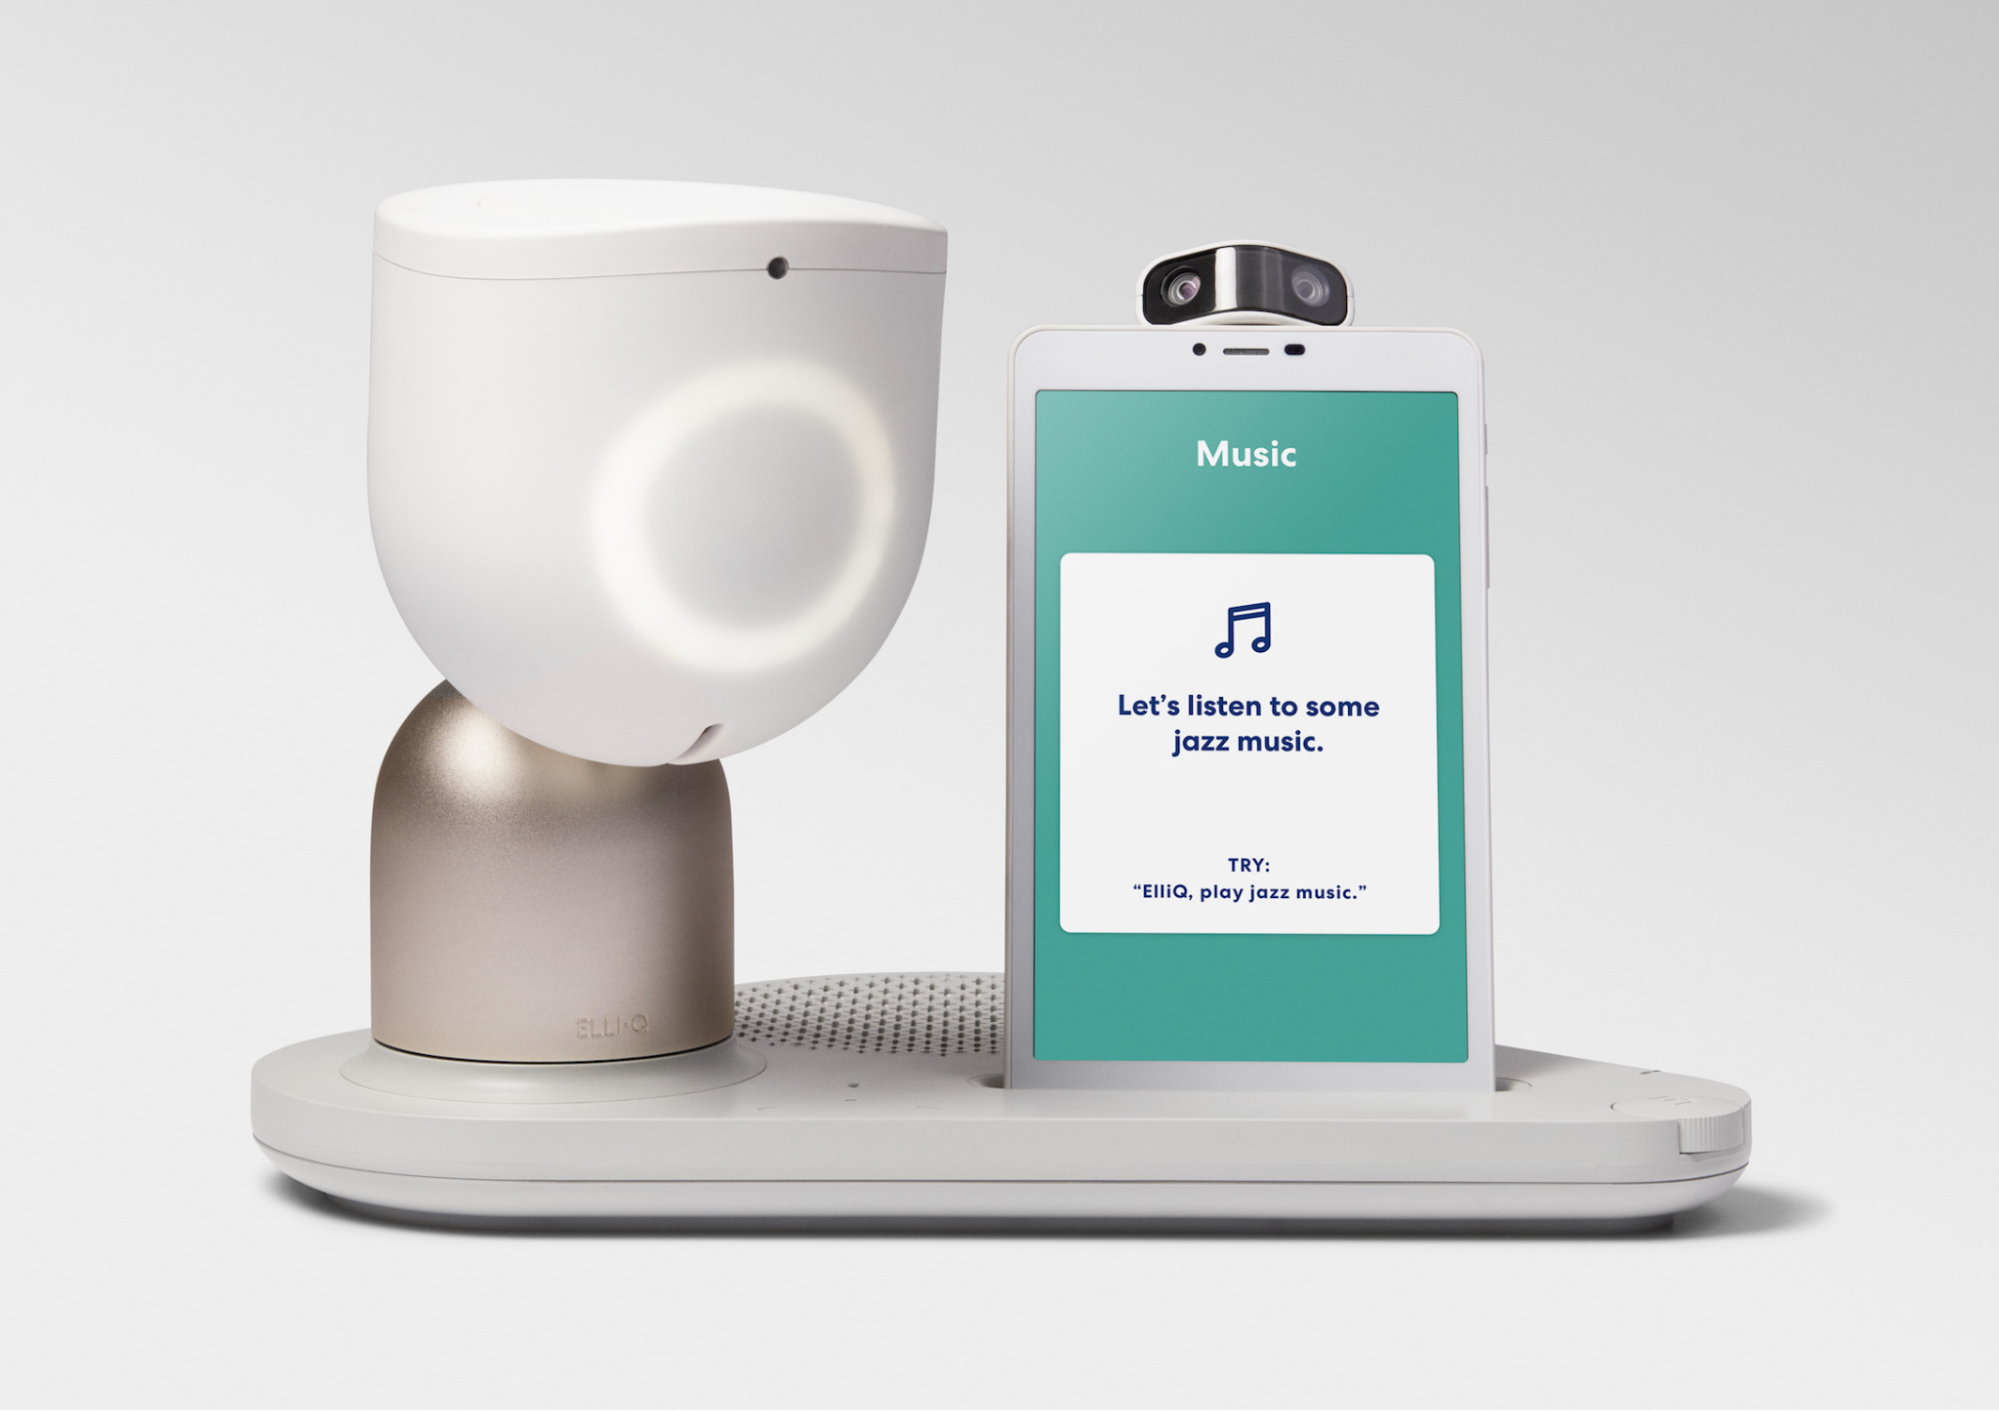
\includegraphics[width=0.6\textwidth]{elliq.png}
    \caption{ElliQ, Source: Adapted from \cite{ieee2023elliq}}
    \label{fig:elliq}
\end{figure}

\newpage
    \item{\bf{LOVOT}}
    \vspace{0.25cm}


LOVOT, developed by Groove X in Japan, is a social robot designed to provide companionship, particularly for older adults experiencing loneliness. Unlike stationary robots, LOVOT features a mobile, pet-like design equipped with AI-driven learning capabilities, allowing it to recognize users, respond to touch, and engage in affectionate interactions. The robot's design incorporates emotional expressiveness, including eye contact, physical warmth, and responsive movement, making it an appealing alternative to traditional social companionship.

A study by Tan et al. \cite{tan2024lovot} examined the impact of LOVOT on single older adults’ social well-being. Participants in the study interacted with LOVOT independently in their homes over a week and later shared their experiences in interviews. The study identified four key themes from these interactions: caring for the social robot, finding companionship, forming meaningful connections, and comparing the robot with traditional pets. Users reported that LOVOT provided emotional comfort and reduced feelings of loneliness, reinforcing the idea that social robots can serve as viable companions for older adults who live alone. Additionally, the participants expressed a preference for LOVOT over pets due to its lower maintenance requirements and its ability to provide companionship without the need for feeding or grooming.

LOVOT's adaptive AI enables it to tailor its behavior to individual users, reinforcing a sense of personal connection. This ability to form unique interactions based on user behavior sets LOVOT apart from other social robots. The study further emphasized the importance of designing robots that foster meaningful social engagement rather than serving as mere technological novelties. These findings suggest that social robots like LOVOT could play a crucial role in mitigating loneliness among aging populations and improving overall well-being.
\end{enumerate}


\begin{figure}[ht]
    \centering
    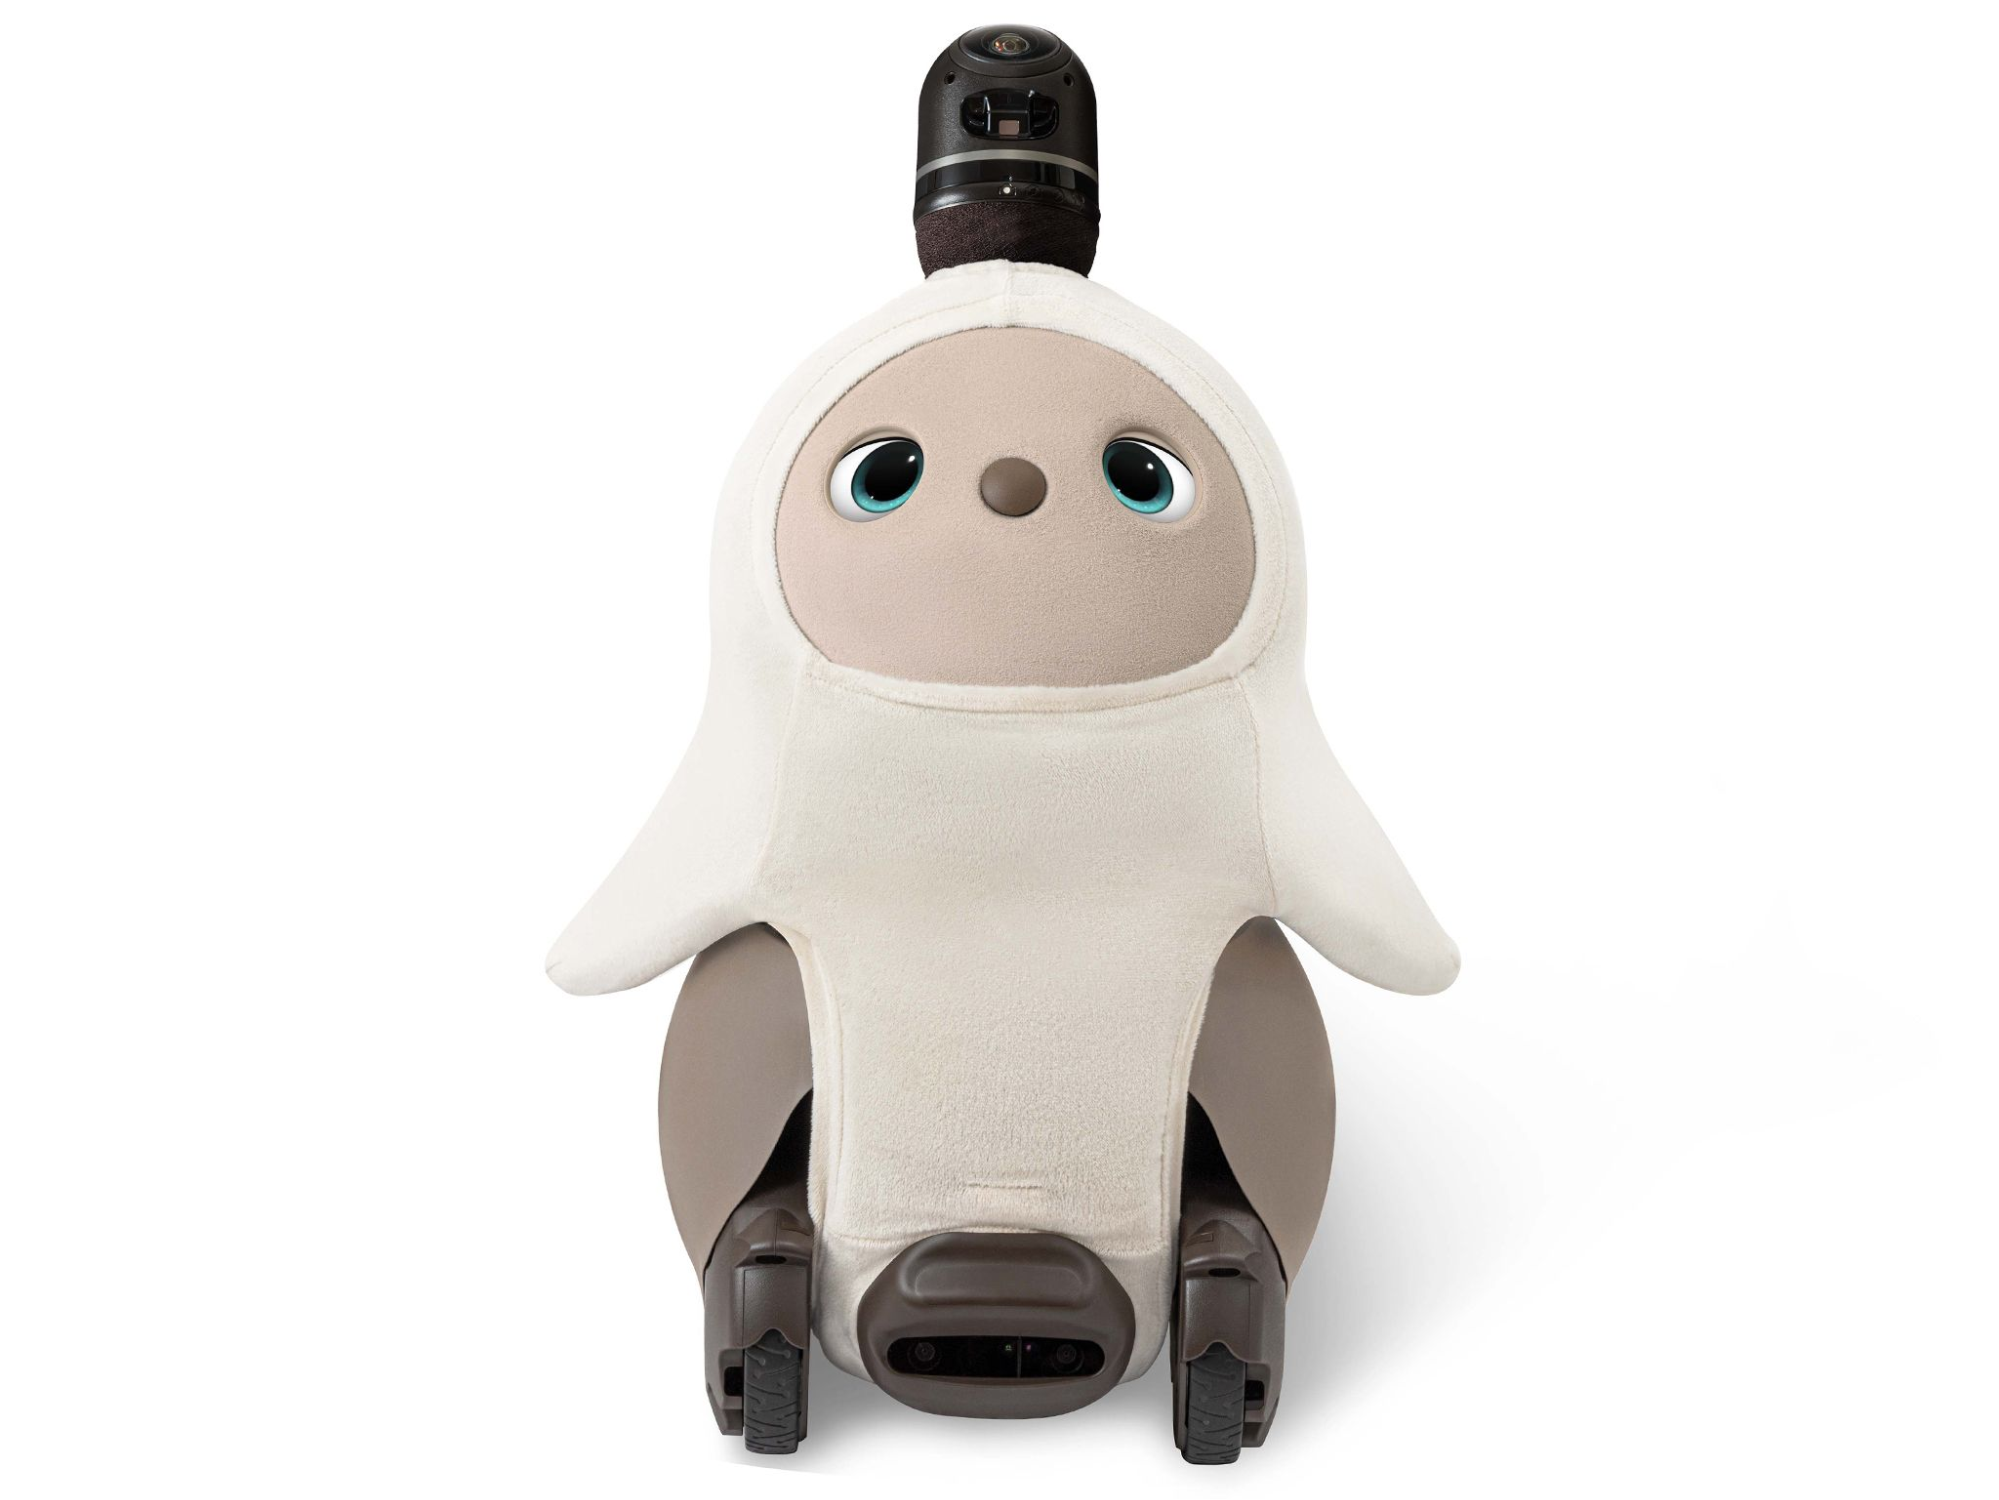
\includegraphics[width=0.6\textwidth]{lovot.png}
    \caption{LOVOT, Source: Adapted from \cite{lovot2024}}
    \label{fig:lovot}
\end{figure}

\subsection{State of the Art}

Bayesian Networks (BNs) are a proven tool for decision-making under uncertainty, as demonstrated by Rothmund et al. \cite{rothmund2021bayesian}, where Dynamic Bayesian Networks (DBNs) were applied to enhance the autonomy of industrial drones. The drones utilized DBNs to infer internal faults, assess environmental conditions, and make proactive decisions to avoid failures while executing independent tasks. By integrating information over time and dynamically updating beliefs, the drones optimized task execution while minimizing risks and the consequences of failures. Our project draws upon similar principles to develop a mental wellness robot designed to promote positivity and reduce stress. Although our robot operates with predefined action bubbles, which are structured interactions tailored to various user emotions, Bayesian Networks can play a vital role in determining which action bubble to deploy based on the user’s current emotional state.

Similar to the drone’s ability to assess environmental conditions, our robot can use a Bayesian Network to infer a user’s emotional state from multiple observable inputs such as facial expressions, vocal tone, and speech patterns. For instance, if vocal cues suggest frustration while facial expressions indicate neutrality, the Bayesian model can combine these observations to probabilistically identify the user’s dominant emotional state. Following the decision-making approach in the drone study, the Bayesian Network can evaluate which predefined action bubble, such as a greeting, playful movement, or verbal feedback, would most effectively promote wellness in the user. By assessing probabilistic relationships between input signals and predefined user emotions, the system ensures that interactions feel relevant and positive.

Emotional indicators are often incomplete or conflicting, such as vocal tone indicating stress while facial expressions suggest calmness. The Bayesian framework excels in such scenarios by integrating prior knowledge and real-time evidence to make confident decisions, ensuring that the robot’s interactions remain meaningful and appropriate. Rothmund et al. \cite{rothmund2021bayesian} emphasized the importance of minimizing risks in decision-making. Similarly, our robot uses Bayesian methods to weigh the likelihood of success for various action bubbles. For example, if the evidence suggests high uncertainty in emotional detection, the robot can select neutral or universally positive interactions to avoid a mismatch between the user’s needs and the robot’s response. The inclusion of Bayesian Networks ensures that the mental wellness robot adapts dynamically to user states, optimizing its responses to enhance emotional support and well-being.
\newpage
\section{Project Development}

This section details the development of Pookie, an AI-driven robot designed to promote mental wellbeing, developed under design supervision from Chula Student Wellness, a platform for free psychological counseling for Chula students. Pookie aims to act as a companion to help alleviate feelings of stress and anxiety, especially in response to future societal concerns like ”Terror Outbursts,” an anxiety-driven phenomenon anticipated to affect Thailand. The project focuses on enhancing positivity and emotional attachment by creating a robot that interacts with users in an empathetic and calming manner.

\subsection{Overview}
\begin{figure}[!htb]
    \centering
    \captionsetup{justification=centering}
    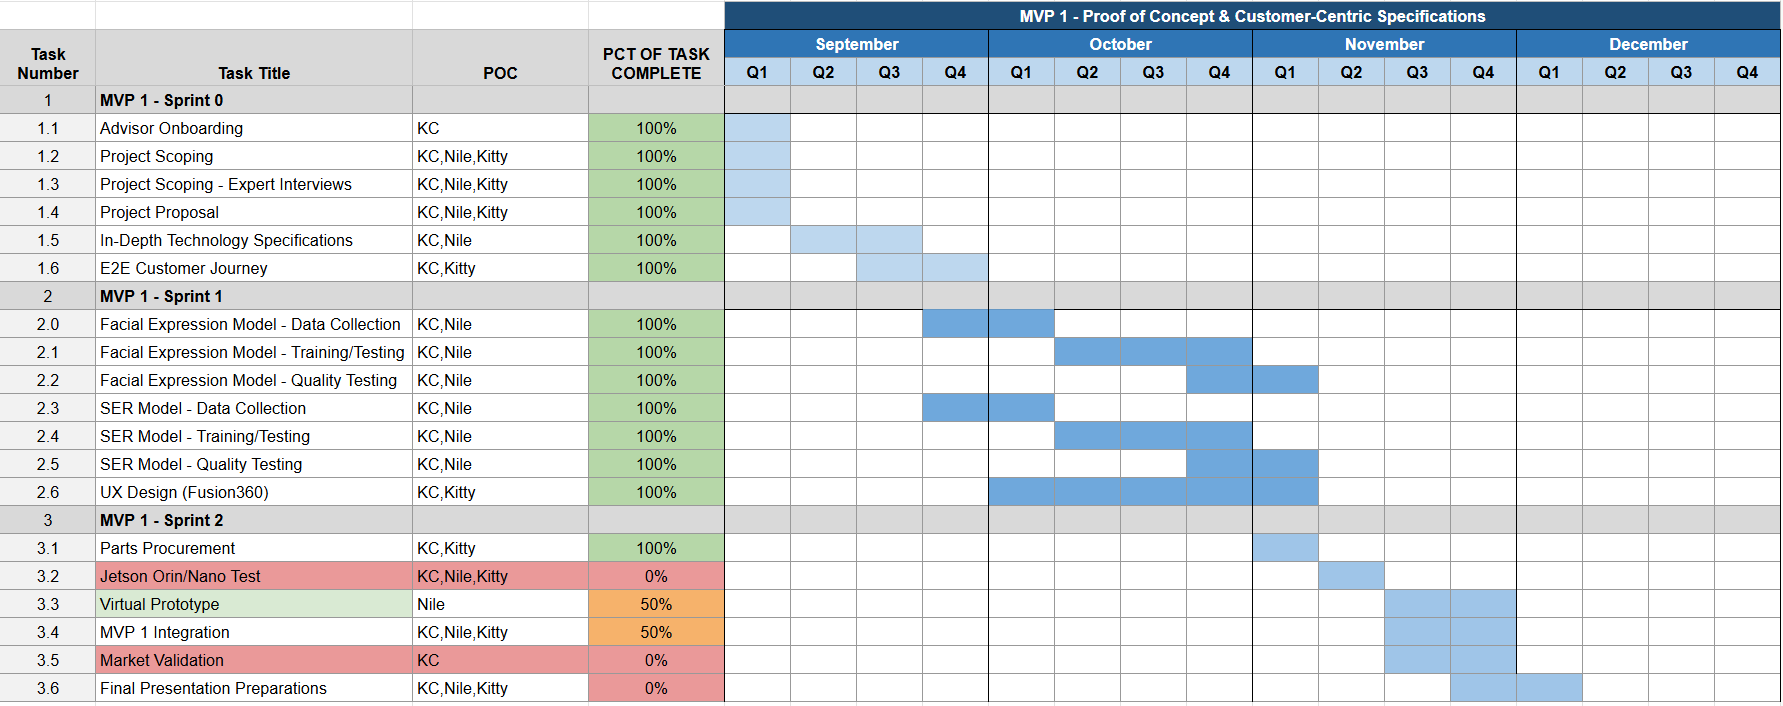
\includegraphics[width=\textwidth]{gantt.png}
    \caption{Project GANTT Chart}
    \label{fig:gantt}
\end{figure}

The project comprises a total of two scopes, one for each semester, where each scope will have its respective expectations. The two scopes are MVP 1 (Proof of Concept) and MVP 2 (Market Prototype). In general, MVP 1 aims to initially collect specifications and design inspiration through primary (expert interviews) and secondary research. Next, a minimum viable product including a working set of AI algorithms, software integration, and CAD mockup was created. On the other hand, MVP 2 aims to elevate the proof of concept to a market prototype, where the software aspects such as AI and integration would be quality tested and dynamic, and the hardware would be readily available for testing.

This report details the implementation of Pookie MVP 1 (Proof of Concept) over the span of four months in semester one. Overall, the project has taken the correct trajectory since conceptualization. As shown in Figure 3, MVP 1 comprises three sprints (Sprint 0, Sprint 1, Sprint 2). In Sprint 0, the team focused on overall product design, reaching out to Dr. Kunparinya Siripanit from Chula Student Wellness for top-down design specifications to accommodate users of general anxiety. Additionally, the team spent time addressing feasibility aspects of the project and literature review, which was discussed in the project proposal. Next, in Sprint 1, the team split into working on their respective tasks, where the software engineering members researched and trained AI models on emotion recognition, including speech emotion recognition and facial emotion recognition, whereas the hardware engineering team focused on developing a mockup of the robot’s physical appearance and acquiring necessary pieces of equipment. Finally, in Sprint 2, the team attempted to integrate all fundamental pieces of software and hardware together. While the project expected integration of software with the Jetson Orin microcomputer, it was recommended by Dr.Paulo instead to focus on developing a virtual prototype, to which a Fusion360 render of the robot’s basic interactions and movements were created. Additionally, the task of \textit{market validation} was also canceled, where initially it was planned that a customer survey and customer interview would be collected to obtain further feedback and refine Pookie’s concept.

\newpage
\subsection{Design Concept}

\subsubsection{Design Reference}

This section illustrates the overall design concept and references for Pookie. Pookie, the emotional wellbeing robot, is conceptualized as a responsive, AI-driven companion designed
to improve mental well-being, specifically catered to customers under the influence of stress and anxiety. To be specific, anxiety in this project is indicated by signs of stress or worry, and the definition of \textit{emotional wellbeing} is \textit{positivity promotion}. It is important to note that the scope of the project, in terms of emotional support, is identified as \textit{promotion}, meaning promotion of positive wellbeing through the use of robotics, rather than \textit{prevention}, which refers to a specific goal of preventing long term issues such as depression or suicide.

With Pookie, it was advised by Dr. Fah Kunpariya (Counseling Psychologist from Chula Student Wellness) to implement an animal-like design with anthropomorphic features. The reason is to reference designs that stimulate a sense of calmness, such as a pet-like design. As such, Pookie resembles a teddy bear, which hopes to stimulate the user with a sense of calmness and childhood nostalgia. After brainstorming and conceptualization, a Fusion360 CAD mockup for Pookie was created. Pookie’s outer shell was 3D printed to hide and house a series of motors, microcontrollers and other necessary electronic components as illustrated in Figure N. Within the scope of this semester, the hardware aspects only comprised a Fusion360 CAD Mockup and virtual prototype. Physical hardware assembly and complete integration was expected to be out of scope, and will begin early next semester in MVP2.

\begin{figure}[!htb]
    \centering
    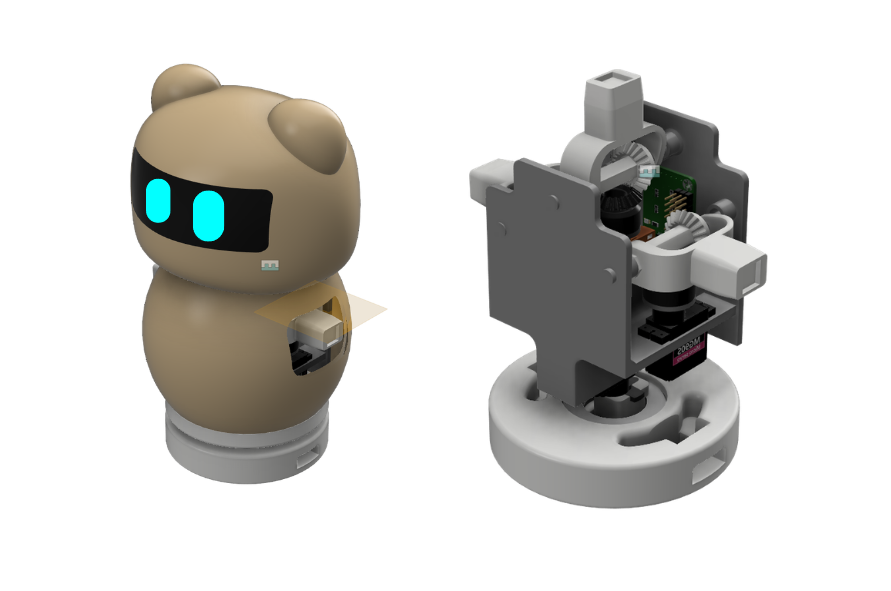
\includegraphics[width=0.7\textwidth]{compare.png}
    \caption{Pookie CAD Mockup. \textit{Left:} Physical Appearance Design, \textit{Right:} Internal Hardware Design.}
    \label{fig:comparison}
\end{figure}

\subsection{Limitations and Scope}

This project aims to develop a proof of concept for an emotional well-being robot, drawing inspiration from existing models such as Kiki. However, there are several limitations and scope considerations for this project:

\begin{itemize}
    \item \textbf{Security:} The primary focus of this project is to create a prototype that demonstrates the feasibility of an emotional well-being robot. As such, the security measures implemented will be at a basic level. Comprehensive security features, including data encryption and advanced user authentication, are beyond the scope of this project.
    \item \textbf{Safety:} While the robot will undergo rigorous testing to ensure fundamental safety in terms of electronics, heat output, and physical design, the scope of safety considerations will be limited to these basic aspects. Detailed safety protocols, including long-term durability and fail-safes for unforeseen hazards, will not be extensively addressed in this prototype phase.
    \item \textbf{Functionality:} The robot will focus on core emotional well-being functionalities, such as basic interaction and mood assessment. Advanced features, such as personalizing therapeutic interventions or integration with external health systems, will not be included in this prototype.
    \item \textbf{User Experience:} The prototype will provide a foundational user experience but may lack the polish and customization of fully developed models. User interface and experience enhancements will be considered in future, scaled development phases.
    \item \textbf{Scalability:} The project will not address scalability concerns for mass production or widespread deployment. The prototype is intended to demonstrate initial concepts and feasibility rather than full scale implementation.
    Integration: This project will not explore extensive integration with other technologies or platforms. The focus will remain on the standalone capabilities of the robot, with minimal emphasis on interoperability with existing systems.
    
\end{itemize}

By acknowledging these limitations and scope considerations, this project sets clear expectations and defines the boundaries of its initial development phase. Future iterations may address these areas in greater detail based on feedback and further research.

\subsection{Software Implementation}
Software implementation for Pookie comprises two key pillars: emotion detection and interaction. Emotion detection is an initiative to incorporate empathy for the customer experience with the robot, using computer vision to analyze facial expressions, as well as speech emotion recognition to analyze tone and pitch. For each AI model, the robot utilizes feature labels of the seven universal emotions (happiness, neutral, sadness, fear, anger, disgust, surprise), which are used as a baseline for many emotion classification tasks, including stress and anxiety detection. In particular, stress and anxiety symptoms are shown to be associated with negative emotions being fear, disgust, and anger, as discussed with Dr.Fah Kunpariya, our psychology advisor. Given predicted emotional status, the robot will be programmed to provide interaction in two forms: verbal and non-verbal. Verbal interactions consist of noises made by the robot, whereas nonverbal interactions comprise physical actions from the robot such as arm movement changes in the LED display resembling its eyes. 
In terms of progress, the goal for semester one was a minimum viable software product, comprising two working AI models and an integration backend that combines the with physical actions and other processing. In terms of AI model implementation, the facial emotion recognition and speech emotion recognition models produced decent results, being more than 50\% accurate in all emotions’ classifications. The integration of these two models uses a server-client architecture to deliver physical interaction, which will be discussed in the software architecture section.

\subsubsection{Process Flowchart}
The process flowchart for Pookie MVP 1 is illustrated in Fig. \ref{fig:flowchart}. Overall, Pookie will detect the user’s face and voice and process the input to induce an action. Based on the emotions detected, such as happy, sad, or negative emotions (inferred as stress), then Pookie will carry out a set of physical actions, including sound, eyes, and actuator. 

\begin{figure}[ht]
    \centering
    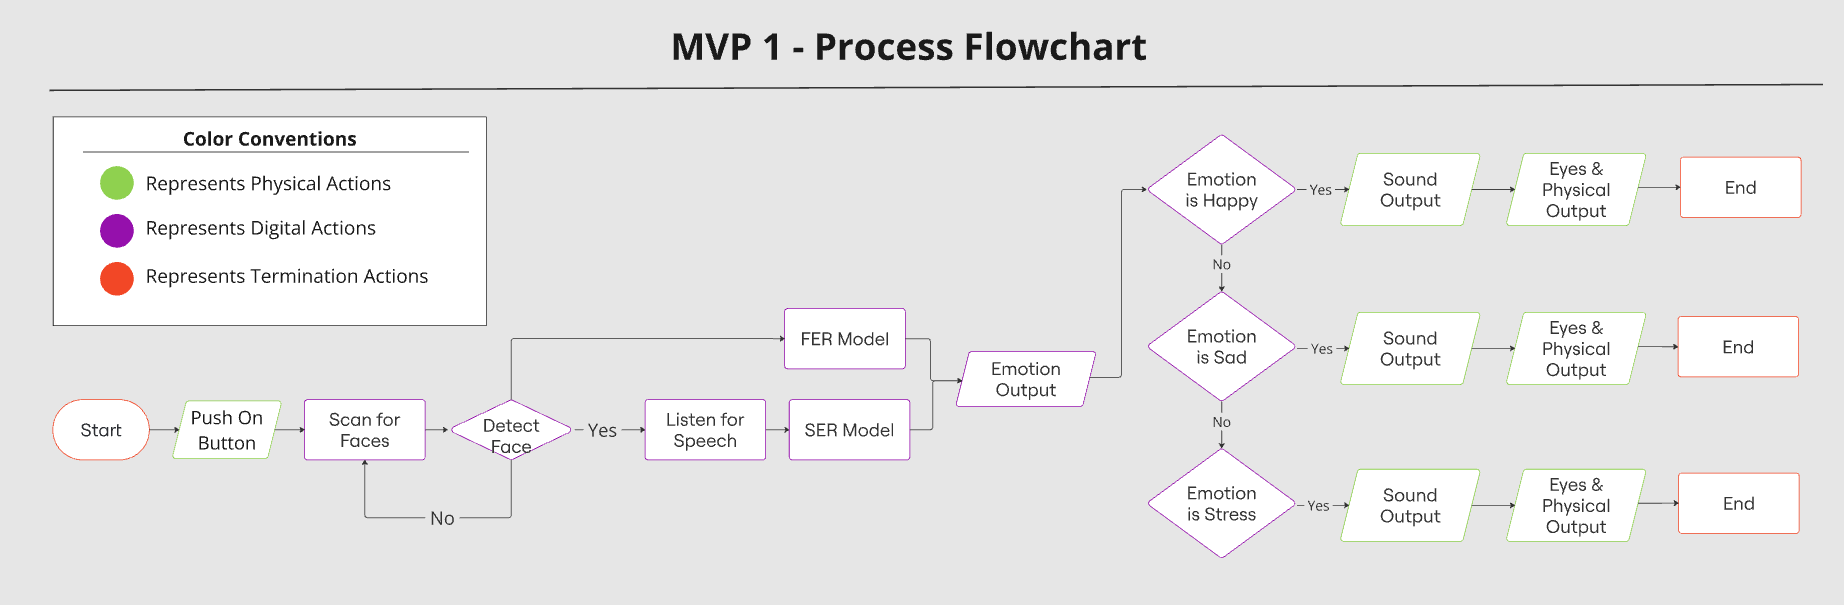
\includegraphics[width=\textwidth]{flowchart.png}
    \caption{MVP 1 Process Flowchart}
    \label{fig:flowchart}
\end{figure}

\subsubsection{Software Architecture and Integration}
To go into further detail on the process flowchart, this section illustrates the solution architecture, involving core technologies used, including servers, clients, libraries and so on.
\textbf{System Overview}

The architecture employs a three-tier structure consisting of:
\begin{itemize}
\item\textbf{Data Acquisition Layer:} Interfaces with sensors and hardware for input collection (e.g., facial images and voice).

\item\textbf{Processing Layer:} Handles emotion analysis using AI models and decision-making algorithms.

\item\textbf{Interaction Layer:} Manages the robot's responses, including audio, visual, and physical movements.
\end{itemize}

This layered design ensures that each module operates independently, facilitating parallel development and easier debugging.

\begin{figure}[ht]
    \centering
    \captionsetup{justification=centering}
    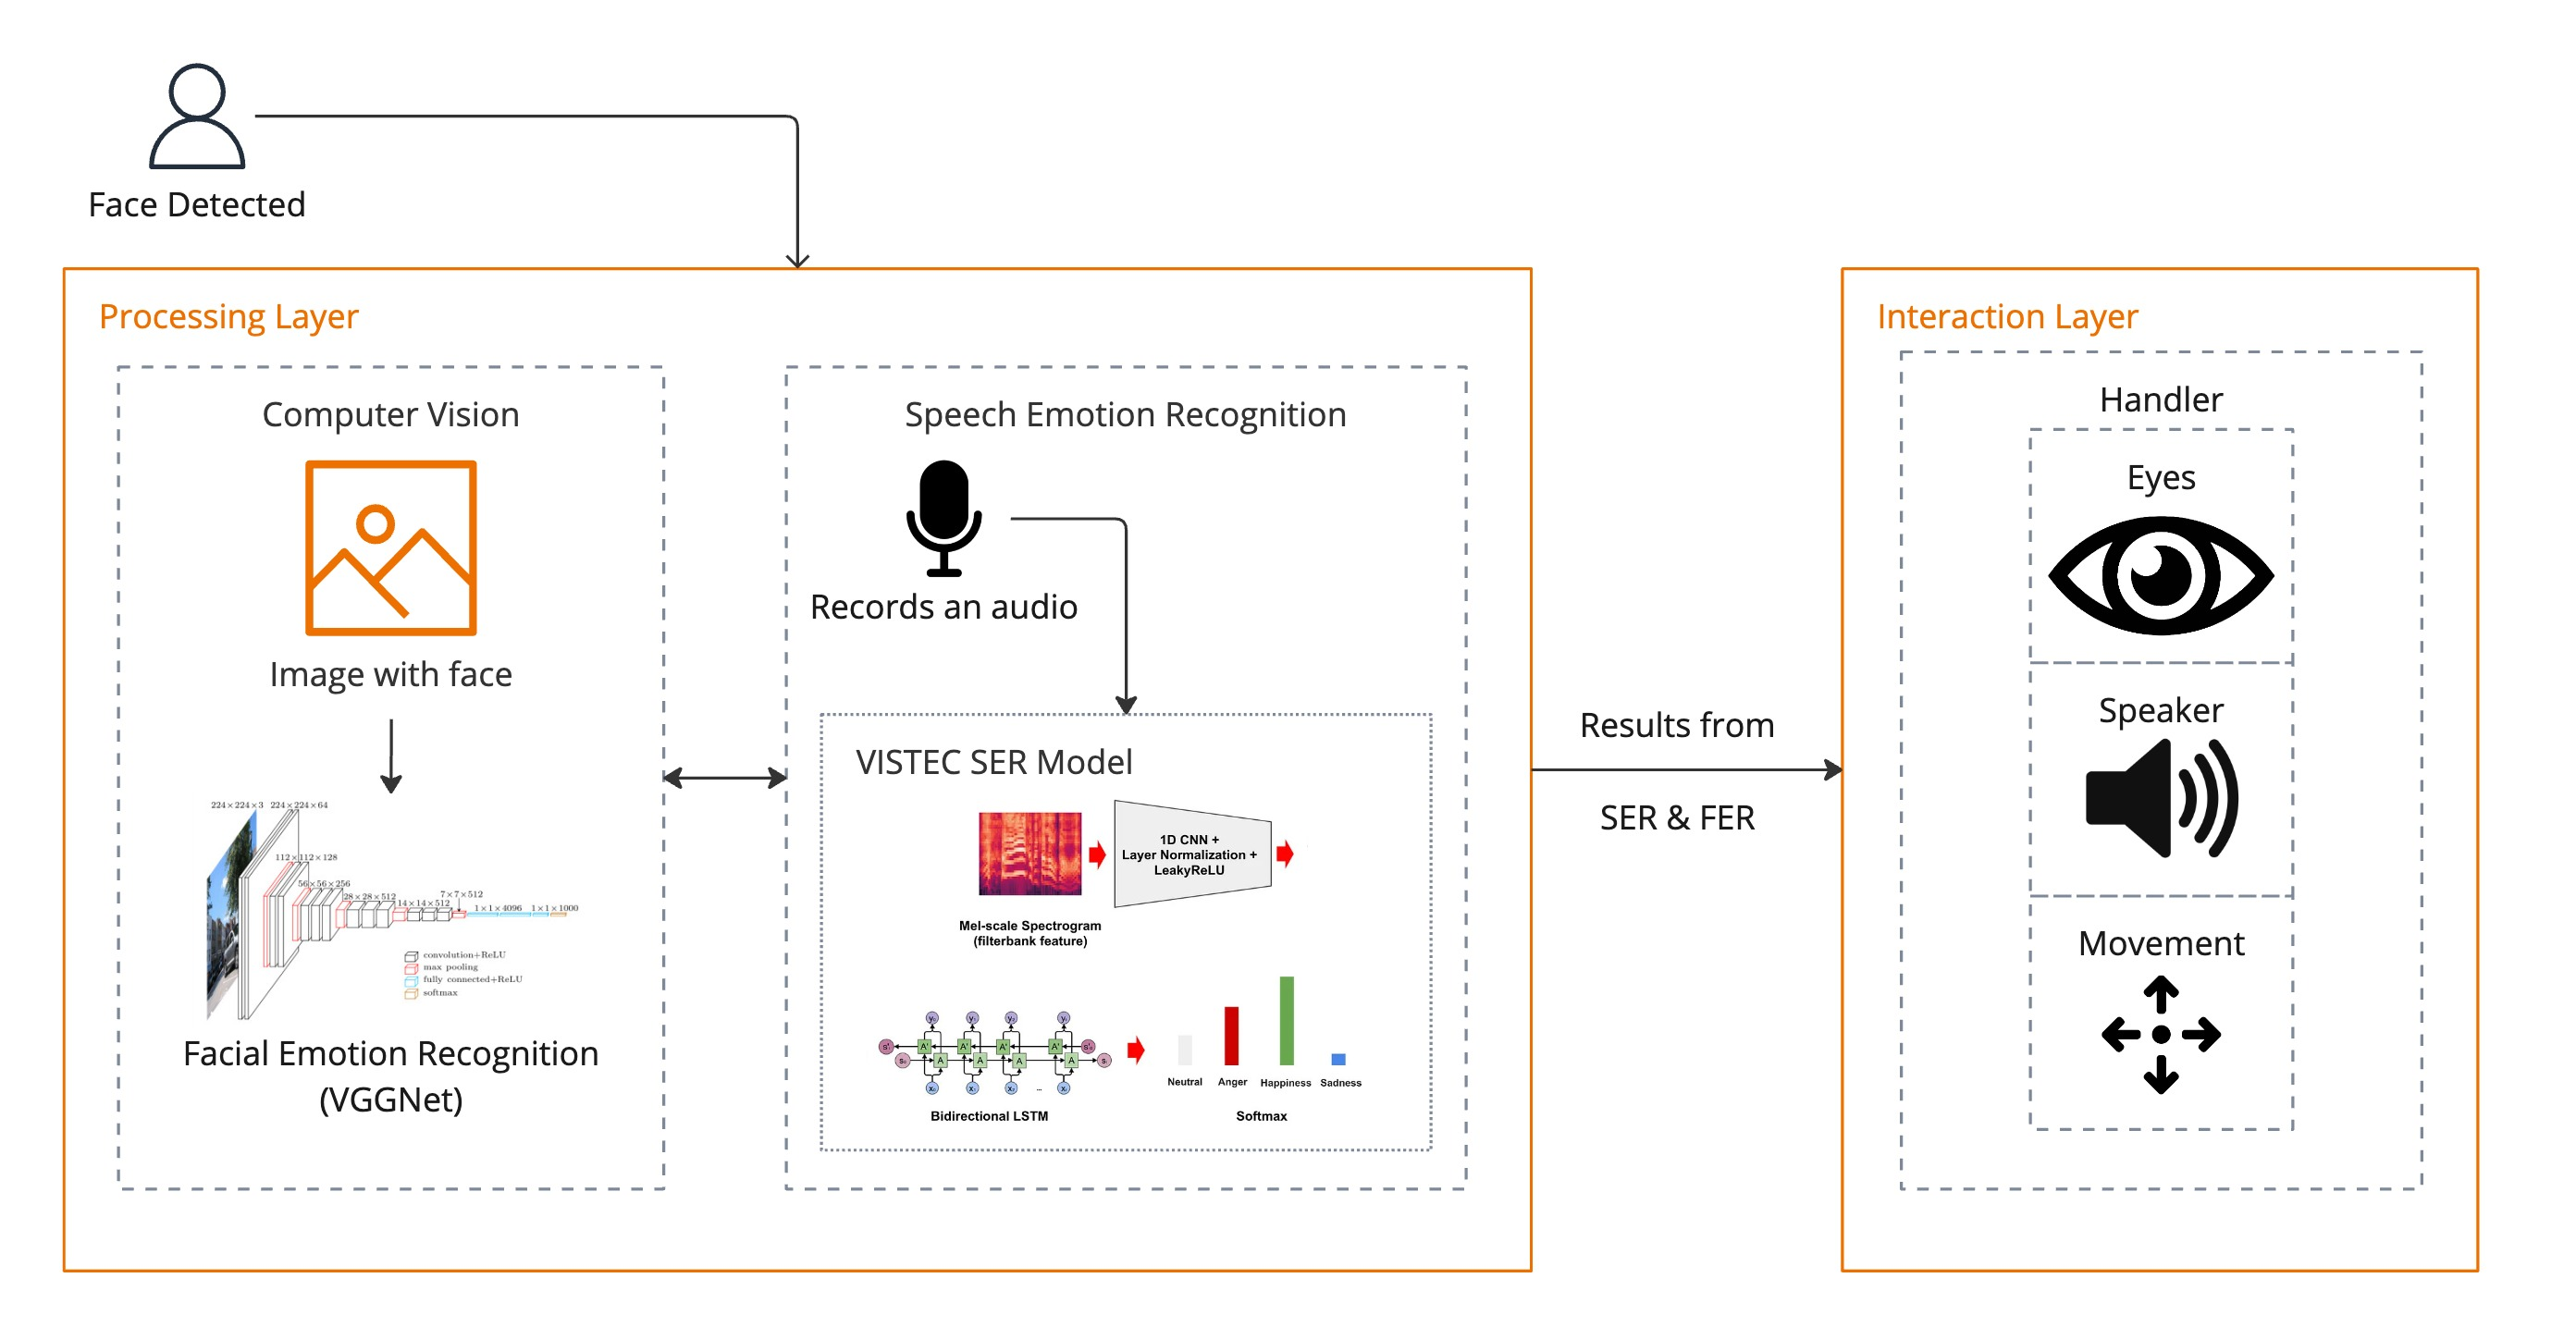
\includegraphics[width=\textwidth]{Flowchart.jpg}
    \caption{Pookie Software Architecture}
    \label{fig:architecture}
\end{figure}

\subsubsection{Key Components}
\begin{enumerate}
    \item\textbf{Emotion Detection Module}

    This module is responsible for identifying the user's emotional state based on facial expressions and speech patterns.
    \begin{itemize}
        \item\textbf{Facial Emotion Recognition (FER):} Utilizes a fine-tuned VGGNet model trained on the Chinese Faces Dataset. It processes real-time video feeds to classify emotions such as happiness, sadness, and stress.
        \item\textbf{Speech Emotion Recognition (SER):} Leverages a pre-trained model developed in collaboration with VISTEC, analyzing voice inputs for tonal features like pitch and intensity to detect emotions.
    \end{itemize}
    Both components output structured emotion data to the Core Integration Framework for further processing.
\item\textbf{Interaction Module}
    
    The Interaction Module generates empathetic responses based on detected emotions:
    \begin{itemize}
        \item\textbf{Verbal Interactions:} Uses pre-recorded audio and tone synthesis to produce comforting sounds or words.
        
        \item\textbf{Non-Verbal Interactions:} Controls physical actions such as arm movements, eye animations on the LED display, and body rotation using servo motors.
    \end{itemize}
\end{enumerate}
        

\subsubsection{Core Integration Framework}


This middleware orchestrates communication between the emotion detection and interaction modules. Key responsibilities include:
\begin{itemize}
    \item Synchronizing data streams from the FER and SER modules.
    \item Deciding responses using a rule-based system or decision tree logic.
    \item Triggering corresponding interaction commands.
\end{itemize}

\subsubsection{Component Interaction}

The interaction between components is depicted in the process flowchart. The steps include:
\begin{enumerate}
    \item\textbf{Data Acquisition:} Real-time inputs (video and audio) are captured using a USB camera and a lavalier microphone.
    \item\textbf{Emotion Detection:} Data is processed by FER and SER modules to output an emotional state.
    \item\textbf{Decision Making:} The Core Integration Framework maps the detected emotion to predefined response rules.
    \item\textbf{Response Execution:} Interaction Module activates verbal and non-verbal responses.
\end{enumerate}

\subsection{Facial Emotion Recognition}
The development of the AI-driven robot incorporates a crucial element: detecting and interpreting user emotions, particularly stress and anxiety, using Facial Emotion Recognition (FER). In particular, stress will be mapped to negative emotions: fear, anger, and disgust.

\subsubsection{Faces Dataset}
The facial expression recognition model was trained on a Chinese Faces Dataset , chosen for its similar characteristics to the hard-to-obtain Thai dataset. Utilizing an intuitive approach to synthetic data generation, the dataset was based on a  \textbf{Chinese Face Dataset with Dynamic Expressions and Diverse Ages Synthesized by Deep Learning} \cite{han-2023}, where a team of researchers created a facial expression image generation model for various Chinese faces belonging to different age groups, genders, and face structure, as shown in Figure \ref{fig:face}, labeled as “Ours”.

\begin{figure}[ht]
    \centering
    \captionsetup{justification=centering}
    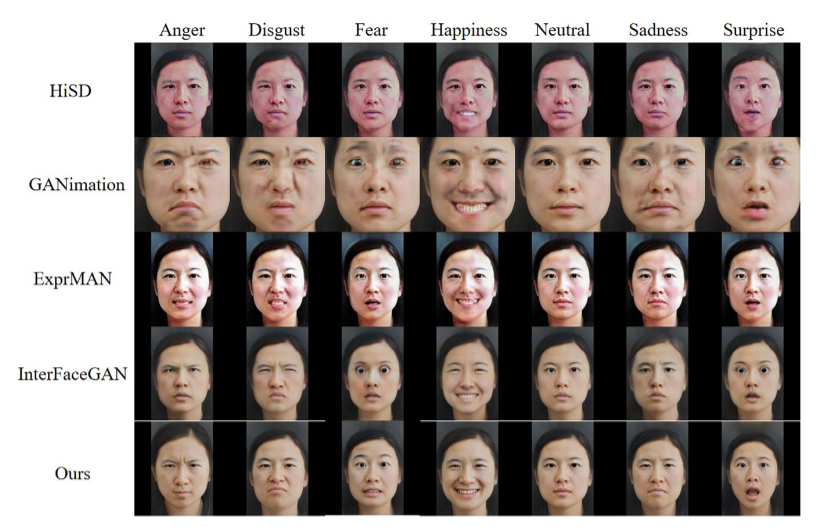
\includegraphics[width=\textwidth]{faces.png}
    \caption{ A Chinese Face Dataset with Dynamic Expressions and Diverse Ages Synthesized. Source: Adapted from \cite{han-2023}}
    \label{fig:face}
\end{figure}


\newpage
\subsubsection{Facial Emotion Recognition Model Development}
Initially, the facial expression recognition model for this project was expected to use a model fine tuning approach over a Chinese Faces Dataset, as it provides the most symmetric resemblance to a Thai dataset, which is difficult to obtain. For our approach, we took a pre-trained model for emotion recognition using VGGNet architecture, then fine tuned the inference layers on a Chinese dataset in order to get more accurate representation for Thai faces. The other layers were frozen, and served as foundation parameters for transfer learning. After multiple versions of the model, however, it could be seen that this approach did not yield great results. As shown in Figure \ref{fig:fer-dev}, the model yielded results far worse than simple guessing, most likely due to inappropriate usage of transfer learning on an already imperfect model.

\begin{figure} [!htb]
    \centering
    \captionsetup{justification=centering}
    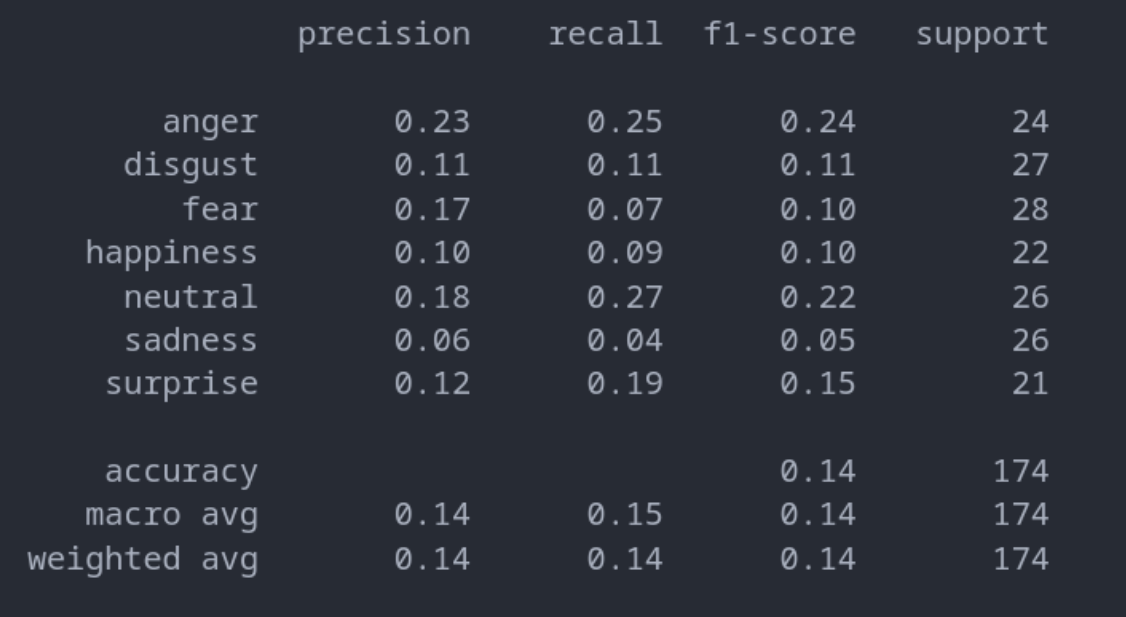
\includegraphics[width=\textwidth]{fer-dev.png}
    \caption{Initial Model Training Results}
    \label{fig:fer-dev}
\end{figure}

\subsubsection{Facial Emotion Recognition Model}
Utilizing a VGGNet \cite{simonyan2015deepconvolutionalnetworkslargescale} architecture (Figure \ref{fig:vgg}) —a multi-layer convolutional neural network renowned for feature extraction and classification, particularly in emotion detection models—the research aimed to develop an accurate facial recognition approach. The Chinese faces dataset was trained over the VGGNet architecture with little hyperparameter tuning.

As seen in the results, the model is great at distinguishing between positive emotions such as happiness or surprise, but it is quite lacking in negative emotions. However, given the scope of the project, where positive and neutral are associated with specific outputs, and negative emotions are all classified as stress, then the model is generally enough to use as a minimum viable product for the rest of the semester.

\begin{figure}
    \centering
    \captionsetup{justification=centering}
    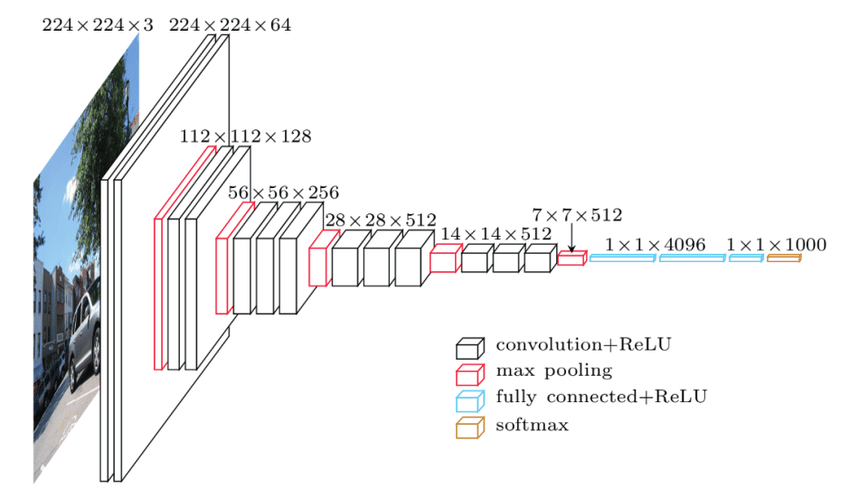
\includegraphics[width=0.8\textwidth]{vgg.png}
    \caption{VGGNet Architecture}
    \label{fig:vgg}
\end{figure}

\begin{figure}
    \centering
    \captionsetup{justification=centering}
    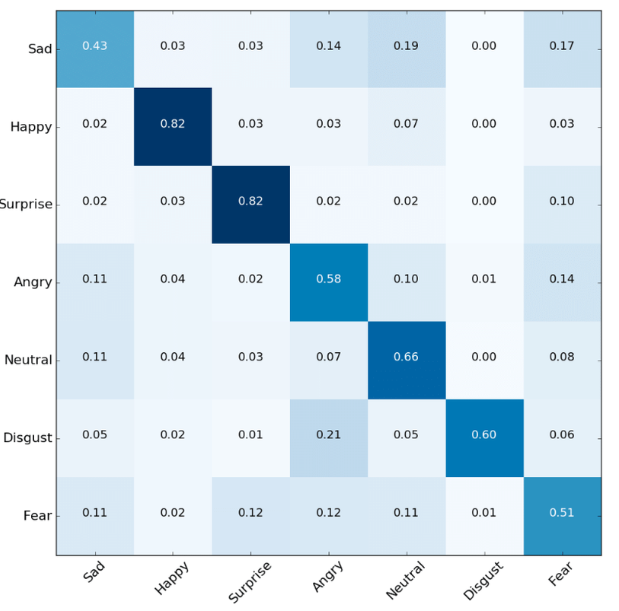
\includegraphics[width=0.8\textwidth]{fer_confusion.png}
    \caption{Validation Set Confusion Matrix}
    \label{fig:fer-con}
\end{figure}

\newpage
\subsection{Speech Emotion Recognition}
A key element of Pookie’s AI is the Speech Emotion Recognition (SER) system, which is used for recognizing the user’s emotions based on vocal patterns. By analyzing factors such as pitch, tone, and intensity, the system detects emotions: neutral, anger, happiness, sadness, and frustration. This section outlines the results and challenges faced during the implementation of the  speech emotion recognition model, starting with relevant datasets and methodologies.

\subsubsection{Speech Emotion Recognition Dataset and Model}
We are utilizing a dataset created by Chulalongkorn University in collaboration with VISTEC, DEPA, and AIS, containing 41 hours and 36 minutes of audio recordings labeled with five emotions: neutral, anger, happiness, sadness, and frustration.
The SER model used within Pookie is also developed by VISTEC which is a speech emotion recognition model based on the aforementioned dataset. 

The confusion matrix visualizes the performance of an emotion recognition model across five classes: neutral, anger, happiness, sadness, and frustration. The diagonal elements indicate correct predictions, with the highest accuracies being for neutral (0.72), anger (0.73), and frustration (0.61). Sadness and happiness show slightly lower accuracies at 0.6 and 0.62, respectively. However, some significant misclassifications occur, such as frustration being confused with sadness (0.31) and happiness being confused with frustration (0.17). The model's weighted accuracy is 66.12\%, while its unweighted accuracy is 65.67\%, reflecting a modest overall performance with some variability in recognizing different emotions accurately.

\begin{figure} [!htb]
    \centering
    \captionsetup{justification=centering}
    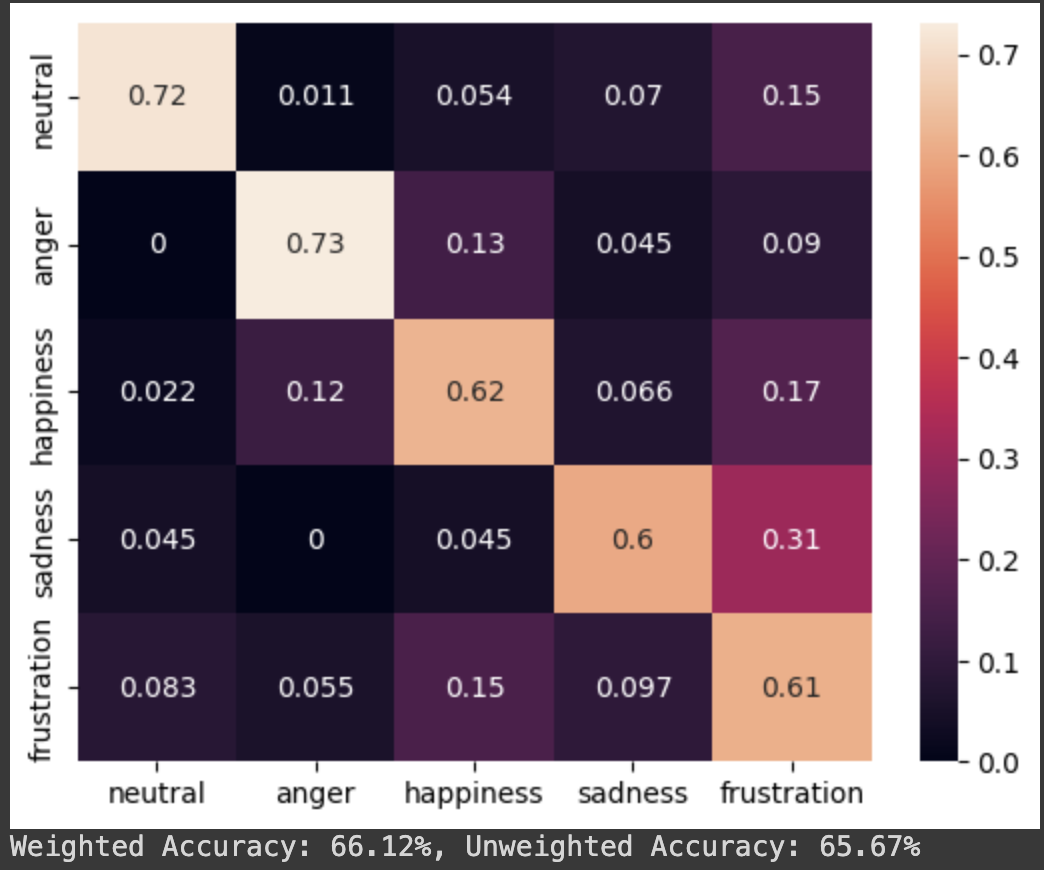
\includegraphics[width=0.8\textwidth]{ser_res.png}
    \caption{SER Confusion Matrix}
    \label{fig:ser-con}
\end{figure}

\newpage
\subsection{Software Challenges}
In this project, multiprocessing was chosen over threading for displaying images with OpenCV's \textbf{\textit{imshow()}} function due to key technical constraints. OpenCV's GUI functions, including \textbf{\textit{imshow()}}, are not thread-safe, which leads to unresponsive windows and crash risks if used in a multithreaded environment. Additionally, Python's Global Interpreter Lock (GIL) limits threading's effectiveness in CPU-bound tasks, preventing full utilization of multicore processors. By using multiprocessing, each process runs independently with its own memory and execution context, allowing true parallelism and better fault isolation. Though multiprocessing introduces overhead, it ensures stable GUI rendering and optimal use of computational resources, making it a better fit for this real-time image processing task. The difference is illustrated in Figure \ref{fig:thread-vs-multiprocessing}.

\begin{figure} [!htb]
    \centering
    \captionsetup{justification=centering}
    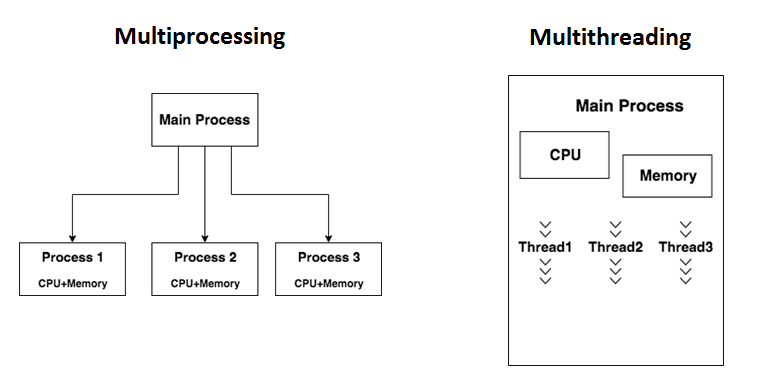
\includegraphics[width=0.8\textwidth]{threadvsmulti.png}
    \caption{Multiprocessing vs Multithreading}
    \label{fig:thread-vs-multiprocessing}
\end{figure}


\newpage
\subsection{Hardware Implementation}
This section details the hardware implementation for Pookie. Overall, the design consists of a robotic shell housing an array of electronic components including the microprocessor, motors, sensors, and so on. A fully functional hardware implementation was not within the scope for this semester, which focused on a basic software proof of concept, and physical design.


\subsubsection{Initial Design}
\begin{enumerate}

    \item\textbf{Outer Shell Design}
    
    In the initial phase, a preliminary design is developed for the outer shell. The design is inspired by Rilakkuma, a well-known Japanese character created by San-X in 2003. Rilakkuma is recognized for its comforting and cute aesthetic, which represents relaxation and embodies the essence of kawaii culture. Its rounded features and laid-back attitude have made it a popular symbol of comfort and appeal \cite{hinka_rilakkuma_history}.
    
    \begin{figure}[ht]
        \centering
        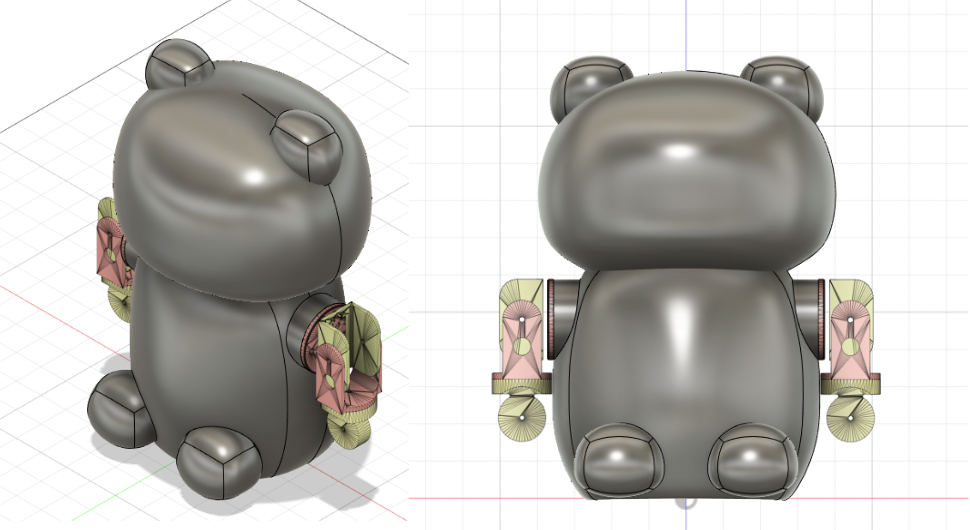
\includegraphics[width=0.6\textwidth]{init-outer.png}
        \caption{Initial Outer Shell Design of Pookie}
        \label{fig:init-outer}
    \end{figure}

    \item\textbf{Inner Shell Mechanism Design}

    The arms are designed to move along the x-axis revolute joint and are powered by CS002 20 Kg servo motors.
    \begin{figure}[ht]
        \centering
        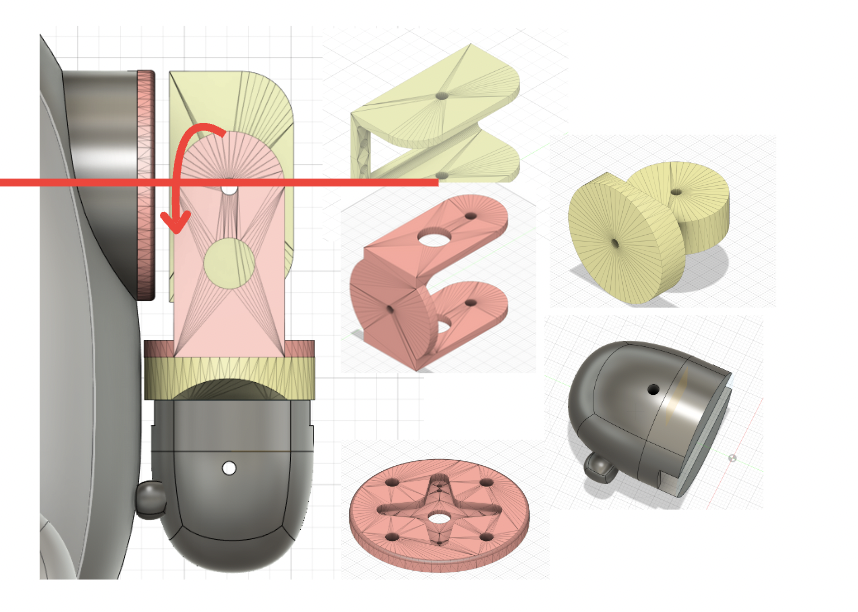
\includegraphics[width=0.6\textwidth]{inner-arm.png}
        \caption{Initial Arm Mechanism of Pookie}
        \label{fig:inner-arm}
    \end{figure}
    
\end{enumerate}
\newpage
\subsubsection{Revised Design}
The revised hardware design of the Pookie robot focuses on anthropomorphic aesthetics, user-centric functionality, seamless mechanical integration, changes in the arm movement axis, and a more compact size.

\begin{figure}[ht]
    \centering
    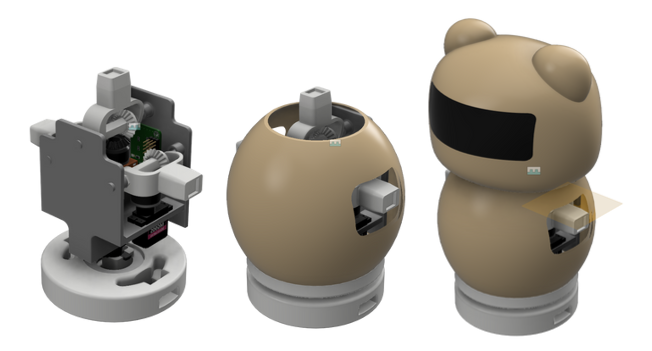
\includegraphics[width=0.8\textwidth]{revised.png}
    \caption{Revised Design of Pookie}
    \label{fig:revised}
\end{figure}

\begin{enumerate}
    \item\textbf{Outer Shell Design}

    The outer shell of Pookie is designed to enclose all internal components in a compact form. It consists of two main sections: the body and the head. The body houses the internal systems, while the head contains an LED screen for displaying the robot's eyes and serves as the mounting point for the head movement mechanism.

\begin{figure}[!ht]
    \centering
    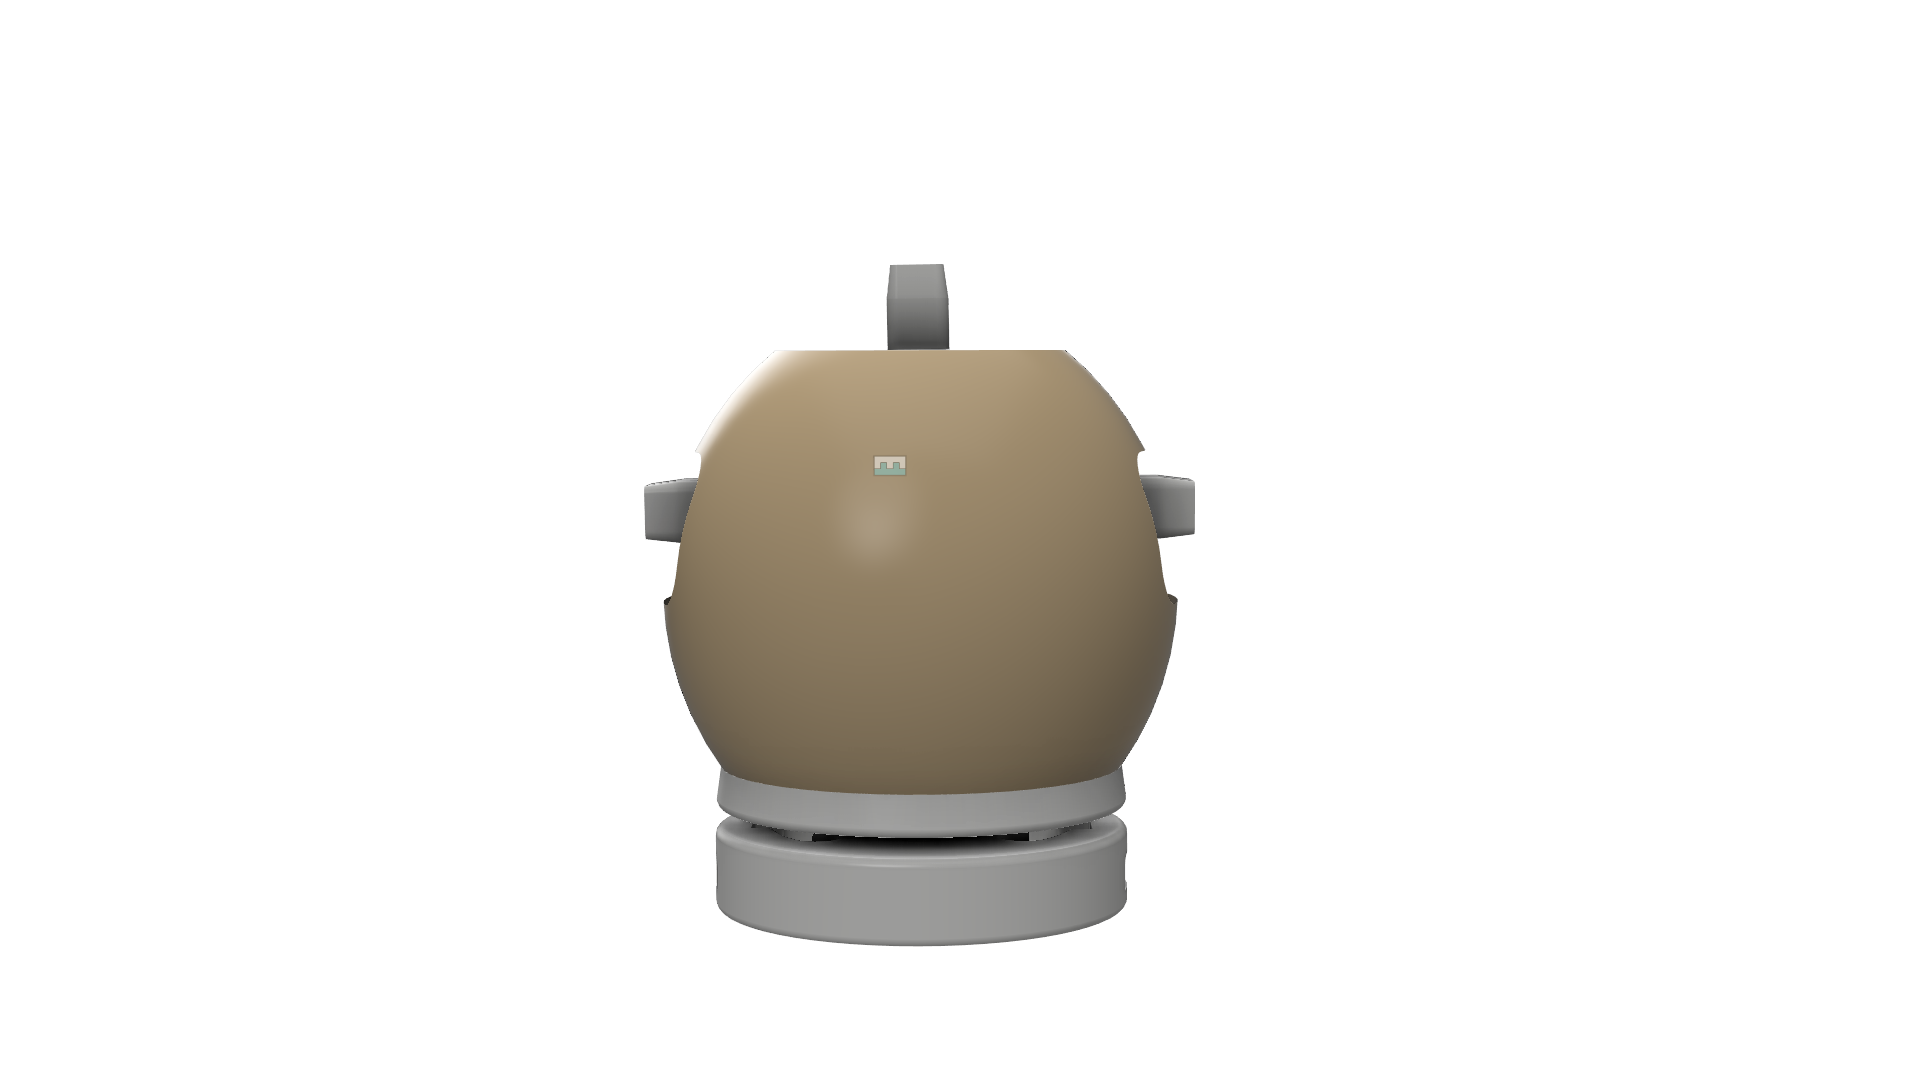
\includegraphics[width=0.8\textwidth]{new_outer.png}
    \caption{Revised Outer Shell Body of Pookie}
    \label{fig:revised_outer}
\end{figure}

\begin{figure}[!ht]
    \centering
    
\includegraphics[width=0.5\textwidth]{new_head.png}
    \caption{Revised Outer Shell Head of Pookie}
    \label{fig:revised_head}
\end{figure}

\newpage
\item\textbf{Inner Shell Mechanism Design}

The movement mechanisms in Pookie include systems for the head, arms, and base. Each actuator is represented as a cylinder, indicating rotational motion driven by MG90s servo motors. The motion occurs along defined axes, with the z-axis primarily supporting rotational movements. 

\begin{figure}[!htb]
    \centering
    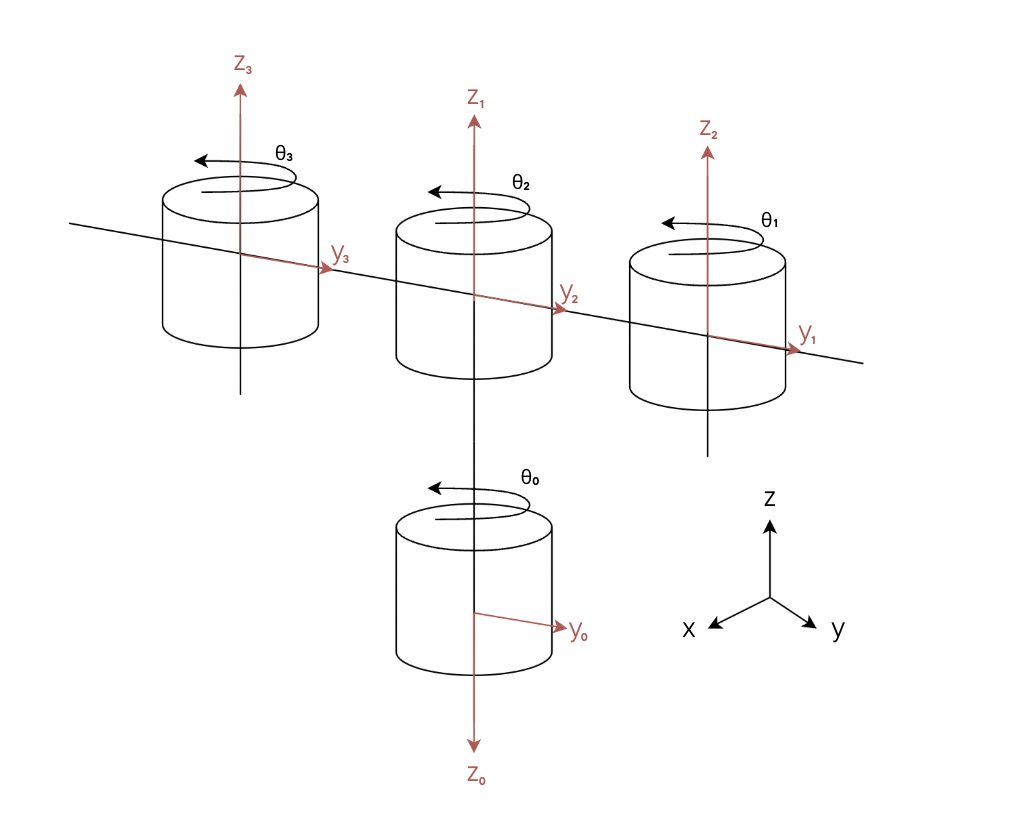
\includegraphics[width=0.7\textwidth]{motion.png}
    \caption{Motion Axes for Pookie's Movement Mechanisms}
    \label{fig:motion}
\end{figure}

Both the head and arm movements use a bevel gear mechanism with a 1:1 transmission powered by MG90s servo motors. This system provides a single degree of freedom along the \textbf{y-axis} revolute joint. A magnet slot at the tip allows easy attachment to the outer shell head, simplifying assembly and maintenance.

\newpage
\begin{figure} [!htb]
    \centering
    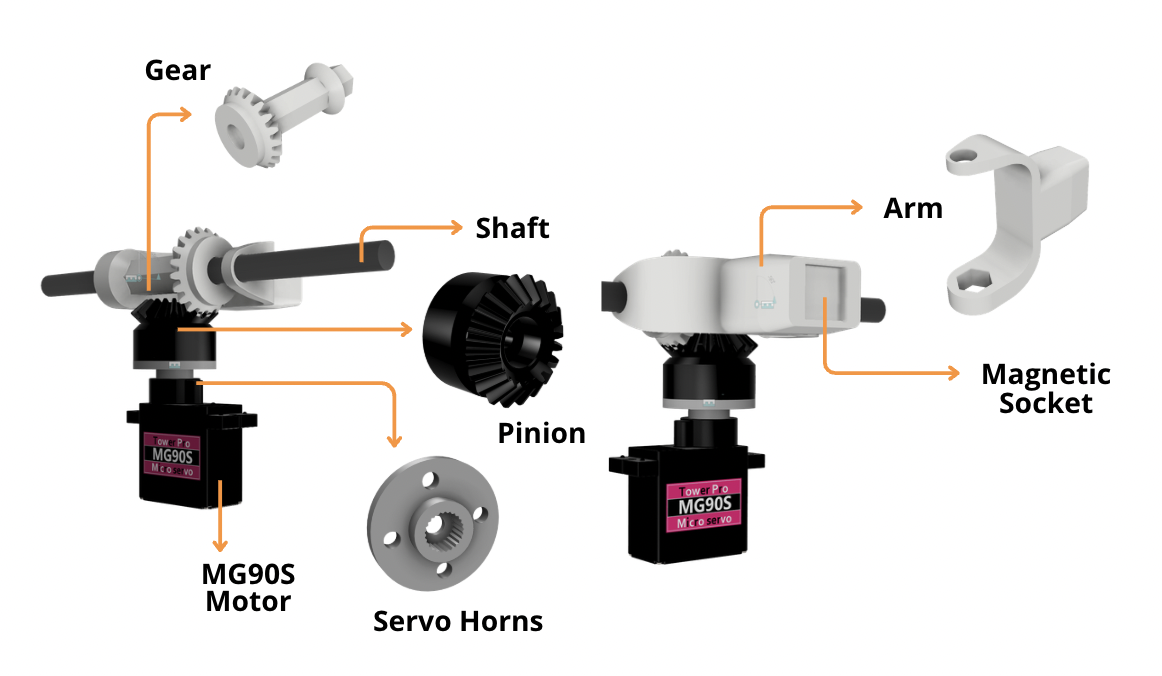
\includegraphics[width=0.7\textwidth]{gear_diagram.png}
    \caption{Components of the Head and Arm Mechanisms}
    \label{fig:components_head_arm}
\end{figure}

The bevel gear mechanism transfers motion from the servo motor to the movement axis efficiently. With a 1:1 transmission ratio, the angular velocity (\(\omega\)) of the driving gear is equal to that of the driven gear. This relationship is expressed as:

\[
\omega_{\text{output}} = \omega_{\text{input}}
\]

where \(\omega_{\text{input}}\) is the angular velocity of the motor, and \(\omega_{\text{output}}\) is the angular velocity of the output gear. Similarly, the angular acceleration (\(\alpha\)) remains unchanged during transmission:

\[
\alpha_{\text{output}} = \alpha_{\text{input}}
\]

This design ensures that the servo motor’s precise control over movement translates directly to the head and arm mechanisms. The torque transmitted by the system is given by:

\[
\tau_{\text{output}} = \tau_{\text{input}}
\]

where \(\tau_{\text{input}}\) is the torque generated by the servo motor. The selection of a 1:1 transmission ratio supports direct coupling, allowing for seamless motion transmission without the need for additional adjustments or gear reduction.

For the base rotation, a bearing-supported system allows full 360-degree rotation along the z-axis. This system incorporates a low-friction bearing assembly, ensuring smooth and precise rotational motion.

\begin{figure}[!htb]
    \centering
    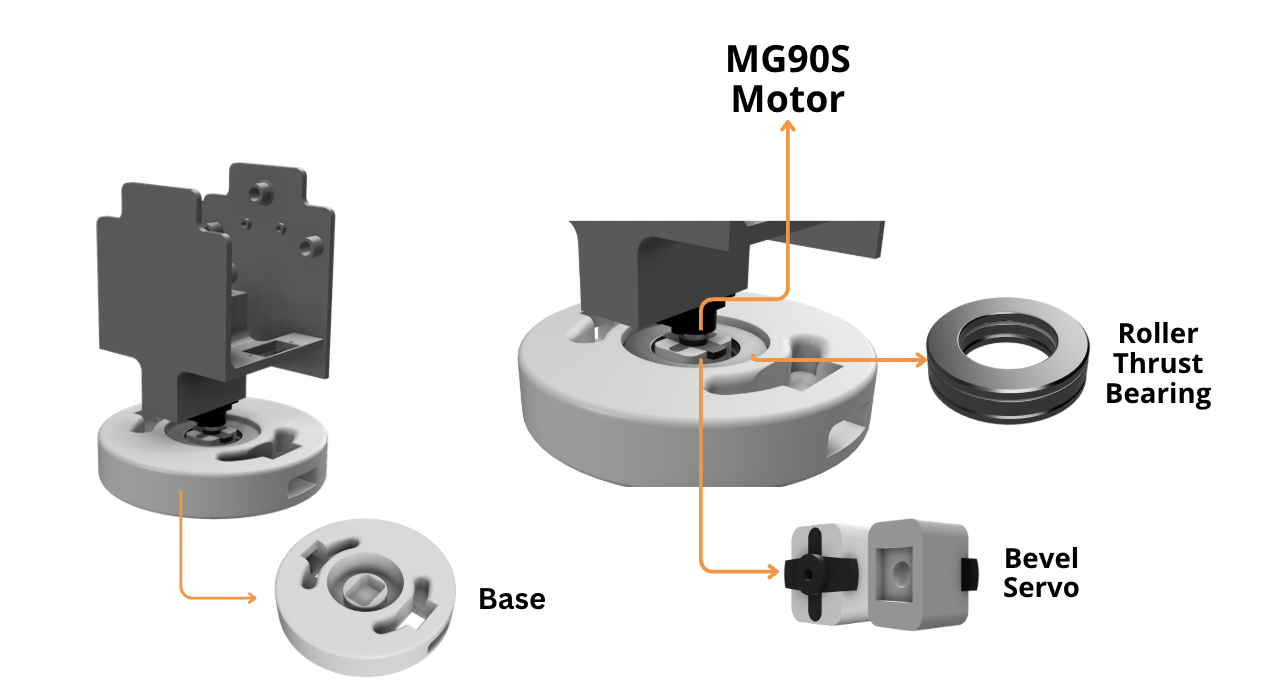
\includegraphics[width=0.7\textwidth]{new_base.png}
    \caption{Components of the Base Mechanism}
    \label{fig:base_comp}
\end{figure}

An armor has been designed to house and support the head, arm, and base rotation mechanisms. It includes compartments for the servo motor and the PWM servo motor driver, as well as openings to facilitate wiring integration. This armor ensures structural integrity and maintains the functionality of all movement mechanisms within Pookie’s compact design.

\begin{figure}[!htb]
    \centering
    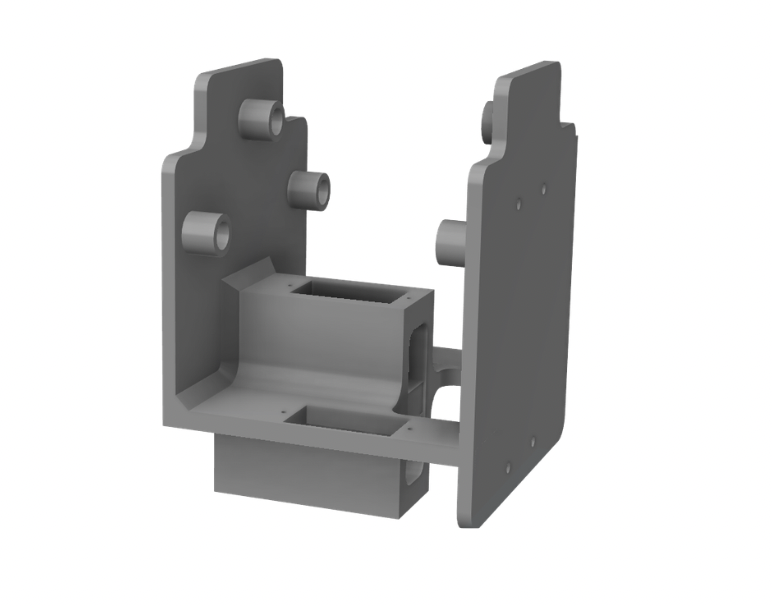
\includegraphics[width=0.7\textwidth]{new_armor.png}
    \caption{Internal Armor Design of Pookie}
    \label{fig:new_armor}
\end{figure}


\end{enumerate}


\newpage
\section{Testing}

This section details the proposed approach to testing Pookie on end users. Overall, the testing phase will be conducted in Semester 2 under the supervision of our psychology advisor, Dr. Fah Kunpariya Siripanit. The testing will comprise 3-4 end users diagnosed with general anxiety. These end users will be volunteers provided by Chula Student Wellness, and in some cases, personal connections. 

The selected users will be given Pookie for a total of seven days to incorporate the robot into their daily lives. Our advisor suggests that seven days is the minimum duration required for a user to develop an emotional attachment. Once they are given the robot, they will complete a questionnaire both before and after the seven-day period to evaluate whether Pookie has had a positive impact on their daily lives. The questions include self-ratings on current anxiety and positivity levels (on a scale from 1-10). 

Since there is no universal interpretation of these scores, a control group (those without access to Pookie) will also answer the questions, allowing the team to establish baseline scores and draw meaningful insights. The key questions are summarized in Table~\ref{table:questions}. It is important to note that while the general rationale for these questions comes from our advisor, the specific wording and execution of the questionnaire will be finalized next year.

\begin{table}[h]
\centering
\caption{List of Questions for Testing}
\label{table:questions}
\begin{tabular}{|l|l|}
\hline
\textbf{Key Questions} & \textbf{Quantitative Metric} \\ \hline
How would you rate your everyday level of anxiety? & Self-rated scale from 1-10 \\ \hline
How would you rate your maximum level of anxiety? & Self-rated scale from 1-10 \\ \hline
How would you rate your everyday level of positivity? & Self-rated scale from 1-10 \\ \hline
How would you rate your maximum level of positivity? & Self-rated scale from 1-10 \\ \hline
\end{tabular}
\end{table}

In regard to security and PDPA compliance, Pookie will require full consent from the end users for the temporary usage of face and voice data. The team is seeking assistance from Chula Regulations to ensure that Pookie adheres to all necessary legal and ethical requirements for testing.

\newpage
\section{Summary and Real Benefit to Industry}
\subsection{Summary}
In summary, the project focuses on developing an emotional wellbeing robot that promotes mental wellness and positivity for users under the influence of stress and anxiety. The robot will utilize technologies such as computer vision and natural language processing to recognize and respond to emotional cues in real time, providing consistent and empathetic support. With a focus on design, interactivity, and empathy, the robot is tailored to meet the needs of Gen Z and younger millennials in promoting mental wellbeing. The project is structured around two academic semesters, employing an agile methodology to deliver two key prototypes, MVP1 (Proof of Concept) and MVP2 (A Fully Functional Design). The development process is guided by insights from Dr. Paulo Fernando Rocha Garcia, Ph.D., Assistant Professor of AI and Robotics at Chulalongkorn University, and Ms. Kunpariya Siripanit, a counseling psychologist at Chulalongkorn University, ensuring that the robot not only meets technical standards but also aligns with mental health principles. This project offers a scalable, innovative solution that addresses the increasing prevalence of anxiety disorders, positioning the robot as a sustainable alternative to traditional mental health support methods. 
\subsection{Benefits Direct Impact on the Industry}
This project will significantly benefit the mental health field, specifically targeting patients with general anxiety and stress, which comprises a massive customer segment. In particular, mental wellbeing robots are an important initiative in countering \textbf{\textit{Terror Outbursts}} in Thailand. By leveraging AI to detect and respond to emotions through facial expressions and voice analysis, these robots can reduce reliance on human intervention in mental positivity promotion. Additionally, the project will enhance service quality by offering consistent promotion of mental well-being, effectively addressing unmet mental health needs. Scalability and Long-Term Value: With recent studies indicating a 55\% increase in anxiety disorders globally from 1990 to 2019, affecting approximately 301 million people worldwide, these robots will become increasingly essential. Their ability to offer real-time, personalized assistance will not only improve individual well-being but also contribute to the long-term sustainability of mental health care systems. While the project will remain in the proof of concept and prototyping stage, it aims to provide an innovative approach to mental wellbeing, potentially scaling to commercial use in the future. 

\newpage
\section{Team Roles and Responsibilities}

Although each student is assigned to a specific component of the project, it is important to recognize that we will collaborate on various aspects. As a result, each role may evolve and shift as the project progresses.
\begin{enumerate}
    \item{\textbf{Kridbhume Chammanard - Project Manager}}
    
    As the Project Manager, Kridbhume Chammanard is responsible for overseeing the entire project, ensuring that all activities align with the established goals and deadlines. Kridbhume will delegate tasks to the project engineers, manage the project timeline, and make necessary adjustments to keep the project on track. Engaging with advisors from ISE and Chula Student Wellness is a key aspect of the role, including providing regular updates and consultations. Kridbhume will streamline the work processes for the project engineers to enhance efficiency and productivity, and will also professionally review and approve all deliverables before submission. Additionally, Kridbhume will oversee the overall project budget, ensuring that expenditures are within allocated limits and that resources are used effectively.
    
    \item{\textbf{Thitaya Divari - Project Engineer, Product Development}}
    
    Thitaya Divari, as the Project Engineer for Product Development, will focus on designing the user experience (UX) of the robot, utilizing CAD software to develop and refine user interfaces. Thitaya will be responsible for sourcing and gathering all necessary hardware components required for the robot’s physical construction, as well as working on the assembly and testing of these components to ensure they meet design specifications. Managing the budget allocated for hardware components and product development activities will be another critical responsibility, including tracking expenses and making adjustments as needed. Thitaya will also prepare detailed documentation of the product development process, including design specifications, component lists, and testing results.
    
    \item{\textbf{Tibet Buramarn - Project Engineer, Software Development}}
    
    In the role of Project Engineer for Software Development, Tibet Buramarn will lead all software development initiatives, including coding, testing, and integrating the robot’s software functionalities. Tibet will implement and manage DevOps practices within the project, ensuring smooth development, deployment, and maintenance of the software. A significant aspect of the role includes ensuring seamless integration of software with hardware components, addressing any compatibility issues, and optimizing performance. Tibet will conduct thorough testing and debugging of the software to identify and resolve issues, ensuring the reliability and functionality of the system.
\end{enumerate}
    

\newpage
\addcontentsline{toc}{section}{References}
\bibliographystyle{IEEEtran}
\bibliography{sections/references}

\end{document}
